\documentclass[a4paper,10pt]{article}
\usepackage[english]{babel}
\usepackage[utf8]{inputenc}
\usepackage{lipsum}
\usepackage[margin=1in,includefoot]{geometry}
\usepackage[hidelinks]{hyperref} % allows clickable references

% Graphics preamble
\usepackage{graphicx} %Allows you to import images
\usepackage{float} % Allows for control of float positions
\graphicspath{{./images/}} % set the path of folder images

% Header and Footer Stuff
\usepackage{fancyhdr}
\pagestyle{fancy}
\fancyfoot{}
\fancyfoot[R]{\thepage}

% Bibliography
\usepackage[backend=bibtex,style=numeric]{biblatex}
\bibliography{Bibliography} 

\begin{document}
%The title page
\begin{titlepage} 
	\begin{center}
	\line(1,0){300}\\
	[0.25in]
	\huge{\bfseries The Graph - First Report}\\
	[2mm]
	\line(1,0){200}\\
	[1cm]
	\textsc{\Large Supervisor: Oliver Baudon}\\
	\textmd{\Large Bordeaux University \\
	May 6, 2019}\\
	[13cm]
	\end{center}
	\begin{flushright}
	\textsc{Member: \\}
	Vo Hung Son \\
	Nguyen Ngoc Nhu Y \\
	Tran Quang Nhat \\
	\end{flushright}
\end{titlepage}
%

%Summary
\pagenumbering{roman}
\section*{Summary}
\addcontentsline{toc}{section}{\numberline{}Summary}

The first that we want to say thank you to Professor Oliver Baudon and Professor Fabien that helping us during the project. This is the first report that we only introduce about the bibliograhy that we use to do this project and we will existing analysis about the library that Professor Oliver Baudon gave us. After that is requirements analysis and objective, architecture and tests. \\
The main purpose of this project is improve the library of the Graph, writing interfaces of the graph.\\
We have four members in our group for Project Graph.

Vo Hung Son - vohungson@gmail.com

Tran Quang Nhat - tranquangnhat2211@gmail.com

Nguyen Hoang Do - hoangdo86@gmail.com

Nguyen Ngoc Nhu Y - nguyenngnhuy@yahoo.com\\
\\
The goal of this project:
\begin{enumerate}
	\item To improve an existing library in Java devoted to manipulate graphs.
	\begin{itemize}
		\item Make the complete review of the library. In particular you may propose modifications linked with version 8 of Java \cite{cite-key5}.
		\item Add javadoc comments \cite{cite-key6} in order to allow the distribution of the library with LGPL license \cite{cite-key7}.
	\end{itemize}
	\item Write a simple graphical interface with JavaFx to create graphs.
	\item Propose an exportation of the graph drawings with TikZ (a language which allows to add graphics in Latex files).
\end{enumerate}
\cleardoublepage
%

%Table of contents
\pagenumbering{arabic}
\tableofcontents
\thispagestyle{empty}
\cleardoublepage
\setcounter{page}{1}
%

%Introduction
\section{Introduction}\label{sec:intro}
	\begin{figure}[H]
		\centering
		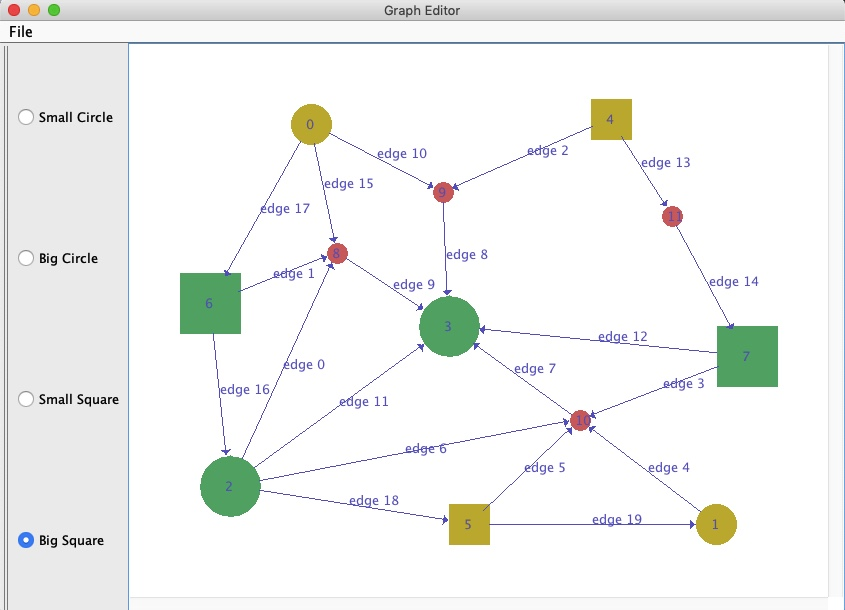
\includegraphics[height = 3in]{image1.jpg}
		\caption[Optional caption]{The Graph}
		\label{fig:Image1}
	\end{figure}
	%Figure \ref{fig:image1} The Graph
Graph Theory is a powerful tool for studying complex combinatorial structures \cite{cite-key1}. But our project only focus to make the interfaces of the graph and use the interfaces that we improved in the existing library and apply them in the JavaFx \cite{cite-key4} graphic program.
We also have to use TikZ language to draw graphic elements in Latex \cite{cite-key2} for the report. Tikz is probably the most complex and powerful tool to create graphic elements in LATEX. In this article some of the basics will be explained: lines, dots, curves, circles, rectangles, etc by means of simple examples.
Almost the knowledge that we use in this project is from the book DaMN \cite{cite-key3}.
%

%Existing Analysis
\section{Existing analysis of The graph}
The source codes that we have 3 packages and main source code.
\subsection{The main source code}
In the main source code, we have these classes: Multigraph, GraphWithEmbedding, DirectedEdge, VertexOrEdgeIterator, VertexOrEdgeIterable...
In the MultiGraph, we have the SubMultiGraph, Edges, Vertices, Graph, SubGraph, ParticialMultiGraph, InducedSubMultiGraph. These classed that we use to make and manage the set of graphs.
The classes VertexOrEdgeIterator, VertexOrEdgeIterable are used for loop vertices and edges.
\subsection{Package Collection}
The package Collection is an Iterator Design pattern that we can loop, append and print...
\subsection{Package Graph}
In this package that we have so many classes.
The class Edges that we can add, remove, clear and iterator.
The class Vertices that we also can add, remove, clear and iterator.
The class Graph that we can add Vertex, remove Vertex, add Edge, remove Edge, check the Vertices are neighbour or not, check the Graph contains Vertex V, check the graph contains Edge E, count the degree of the graph and we also can remove all vertices and all edges.
The class MultiGraph and SubMultiGraph have the same functions with the class Graph but they have more sets of the graph.
There are three interfaces here: PartialGraph, InducedSubGraph, SubGraph.
There are these classes VertexOrEdgeIterator, VertexOrEdgeIterable. This is an Iterator design pattern that use for Vertex and Edge.
\subsection{Package Util}
This package have many classes like: Graphs, Vizing, Conjecture, ShortestPathsMatrices, NegativeEdgeException, Lamda, Position, DepthFirstSearchDataImpl, RandomGraphVietnam, RandomGraph, FlowResults, NegativeCircuitException, K Coloring.
Here applies some algorithms like Coloring, Shortest Paths, Depth First Search, Flow Network...
In the flow network that we show the Maximum Flow and minimum cut of the network.
Especially in the class Graphs have so many algorithm functions inside like: breathFirstSearch, dijkstra algorithm, bellmanFord algorithm, floydWarshall, kruskal, prim, fordFulkerson...
%

%Requirement Analysis
\section{Proposed system}
\subsection{Overview}
Implement a simple application which allow creating the graphs.
Implement graphic interfaces to creating the graphs.
Improve the code of the existed library.
Propose a exportation of the graph drawings with TikZ (a language which allow to add graphics in Latex files).
\subsection{Functional requirements}
\subsubsection{Graph interfaces}
 - Design user interfaces which allow users can create the graphs that user want.
 \paragraph{} example:
 \subparagraph{} - User can create a graph by clicking left mouse to create the vertices and after that drag the left mouse from any a vertice to the other vertice to create a edge after drop the left mouse.
 \subparagraph{}  - User can input the number of vertices and the edges and after that user click button create graph, the application will create a graph which user inputed.
 \subparagraph{}  This two basic options for user interface creating the graphs.

\paragraph{}- Design a user interface for solve the shortest path,flow problem.

 \subparagraph{}example: 
 \subparagraph{} - User input the start vertice and the end vertice and after that clicking shortest path button that the application will calculate and print the shortest path in graph interface by highlight the edges with red color.

\subsubsection{Improve and Optimize the performence of algorithms in library}

\begin{enumerate}
\item What things which need to Improve and Optimize.
\begin{itemize}
\item Review and remove the duplicate code.
\item Add comment javadoc for the functions.
\item Add more the unit test for detail test functions which added and improved.
\end{itemize}
\end{enumerate}

\subsection{Nonfunctional requirements}
\subsubsection{Usability}
\begin{enumerate}
\item This is a desktop application.
\begin{itemize}
\item Runnable on the difference Operating System: Windows,linux or any machine have installed Java virtual machine.
\item Optimize the space memory of the application.
\item The user interface should be simple as posible as and friendly with the user.
\item User can choose the algorithms which user want the application do example: Dijktra or Bellman-Ford for the shortest path problem.
\item Improve and optimize the performence of application.

\end{itemize}
\end{enumerate}
\subsubsection{Reliability}

\begin{enumerate}
\item Making sure of Reliability
\begin{itemize}
\item Components of the project code will be tested alongside the implementation phase to ensure that they are functional. 
\item Final, integrated project Code will be tested with JUnit to ensure that greater than or equal to 80\% of the integrated code is covered at run-time, and is functioning properly. The remaining 20\% will be inspected through manual testing to ensure the highest chance of being quality code.


\end{itemize}
\end{enumerate}
\subsubsection{Performance}
\begin{enumerate}
\item Making sure of Performance
\begin{itemize}
\item Drag and drop of the tiles must be smooth without graphical lagging. 
\item The time of finding the shortest path must be fast (under 5 seconds).
\end{itemize}
\end{enumerate}

\subsubsection{Supportability}
\begin{enumerate}
\item Making sure of Supportability
\begin{itemize}
\item The application must not be platform dependent, i.e., it should be able to run on any platform supporting JAVA.
\end{itemize}
\end{enumerate}

\subsubsection{Implementation}
\begin{enumerate}
\item Making sure of Implementation
\begin{itemize}
\item Project will be implemented in JAVA 8.
\item All project graphical user interfaces will be created using JavaFX.
\end{itemize}
\end{enumerate}
\subsubsection{Interface}


\subsection{System models}
\subsubsection{Use case model}
\paragraph{}
\begin{tabular}{|r|l|}
\hline
Name: & Find The Shortest Path Of Graph \\
\hline
Actor & User \\
\hline
Entry Conditions: & Application is running. \\
\hline
Flow of Events: & 1. User choose the algorithm which want to apply. \\


& 2. System remember the algorithm which user chose.  \\
& 3. User click find shortest path button  \\
& 4. System calculate and give the result. System will highlight with red color  \\
& for the edges in the shortest path. \\
\hline
Exit Conditions: & The application is now in a new state. \\
\hline
\end{tabular}
\paragraph{}
\begin{tabular}{|r|l|}
\hline
Name: & Draw Vertices \\
\hline
Actor & User \\
\hline
Entry Conditions: & Application is running. \\
\hline
Flow of Events: & 1. User choose type of vertice which want to draw. \\


& 2. System remember the type which user chose.  \\
& 3. User click mouse left button on panel.  \\
& 4. System will draw a vertice on the panel.  \\
\hline
Exit Conditions: & The application is now in a new state. \\
\hline

\end{tabular}

\paragraph{}
\begin{tabular}{|r|l|}
\hline
Name: & Draw Edges \\
\hline
Actor & User \\
\hline
Entry Conditions: & Application is running. \\
\hline
Flow of Events: & 1. User press left button mouse and alt key on one the start vertices \\
& 2. User drag mouse to the end vertice to create a edge by release left button\\
& 3. System will create a edge with start and end vertices\\
\hline
Exit Conditions: & The application is now in a new state. \\
\hline

\end{tabular}
\paragraph{}
\begin{tabular}{|r|l|}
\hline
Name: & Delete Edges \\
\hline
Actor & User \\
\hline
Entry Conditions: & Application is running. \\
\hline
Flow of Events: & 1. User click right button mouse on edge which user want to delete. \\
& 2. System delete edge user clicked right mouse button  \\

\hline
Exit Conditions: & The application is now in a new state. \\
\hline

\end{tabular}
\paragraph{}
\begin{tabular}{|r|l|}
\hline
Name: & Delete Vertices \\
\hline
Actor & User \\
\hline
Entry Conditions: & Application is running. \\
\hline
Flow of Events: & 1. User click right button mouse on vertices which user want to delete. \\
& 2. System delete vertices which user clicked right mouse button  \\
\hline
Exit Conditions: & The application is now in a new state. \\
\hline

\end{tabular}
\paragraph{}

\begin{tabular}{|r|l|}
\hline
Name: & Move Vertices \\
\hline
Actor & User \\
\hline
Entry Conditions: & Application is running. \\
\hline
Flow of Events: & 1. User press left button mouse on vertices which user want to move. \\
& 2. user drag mouse to move the vertices to position where user want  \\

& 3. System move the vertices  \\
\hline
Exit Conditions: & The application is now in a new state. \\
\hline

\end{tabular}
\subsubsection{Object model}
\begin{figure}[H]
		\centering
		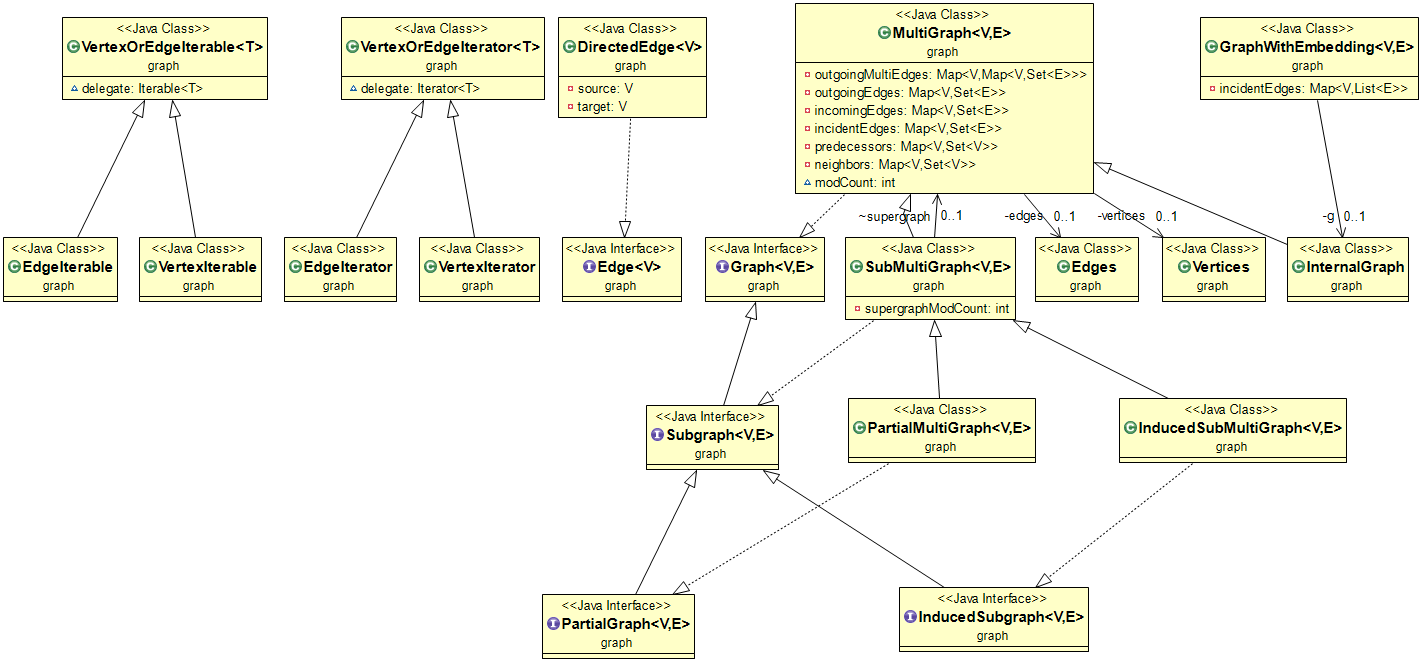
\includegraphics[height = 3in]{1main.png}
		\caption[Optional caption]{Main}
		\label{fig:1main}
	\end{figure}
	%Figure \ref{fig:image1} The Graph
	
	\begin{figure}[H]
		\centering
		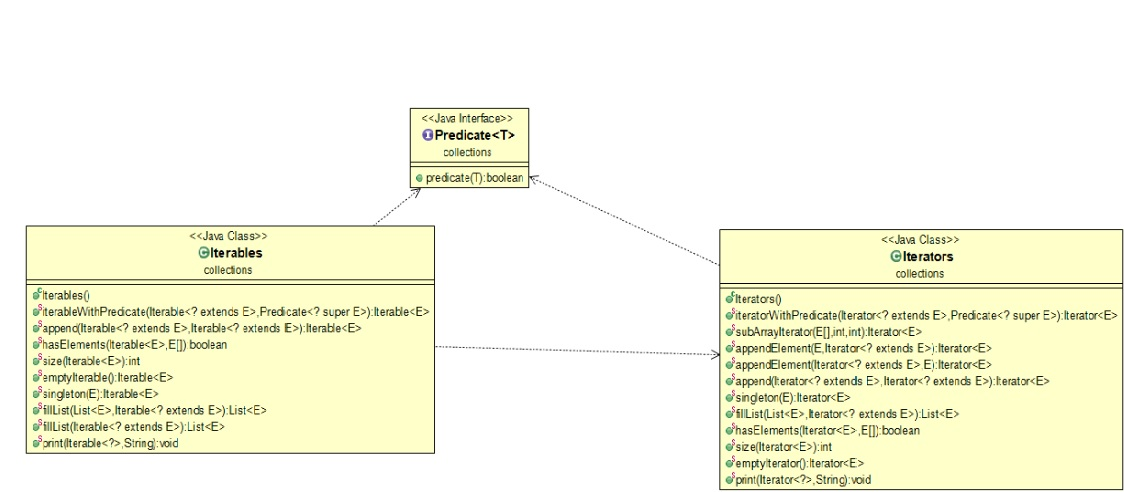
\includegraphics[height = 3in]{f3_edit.jpg}
		\caption[Optional caption]{Package Collection}
		\label{fig:1main}
	\end{figure}
	%Figure \ref{fig:2packagecollection} The Graph
	
	\begin{figure}[H]
		\centering
		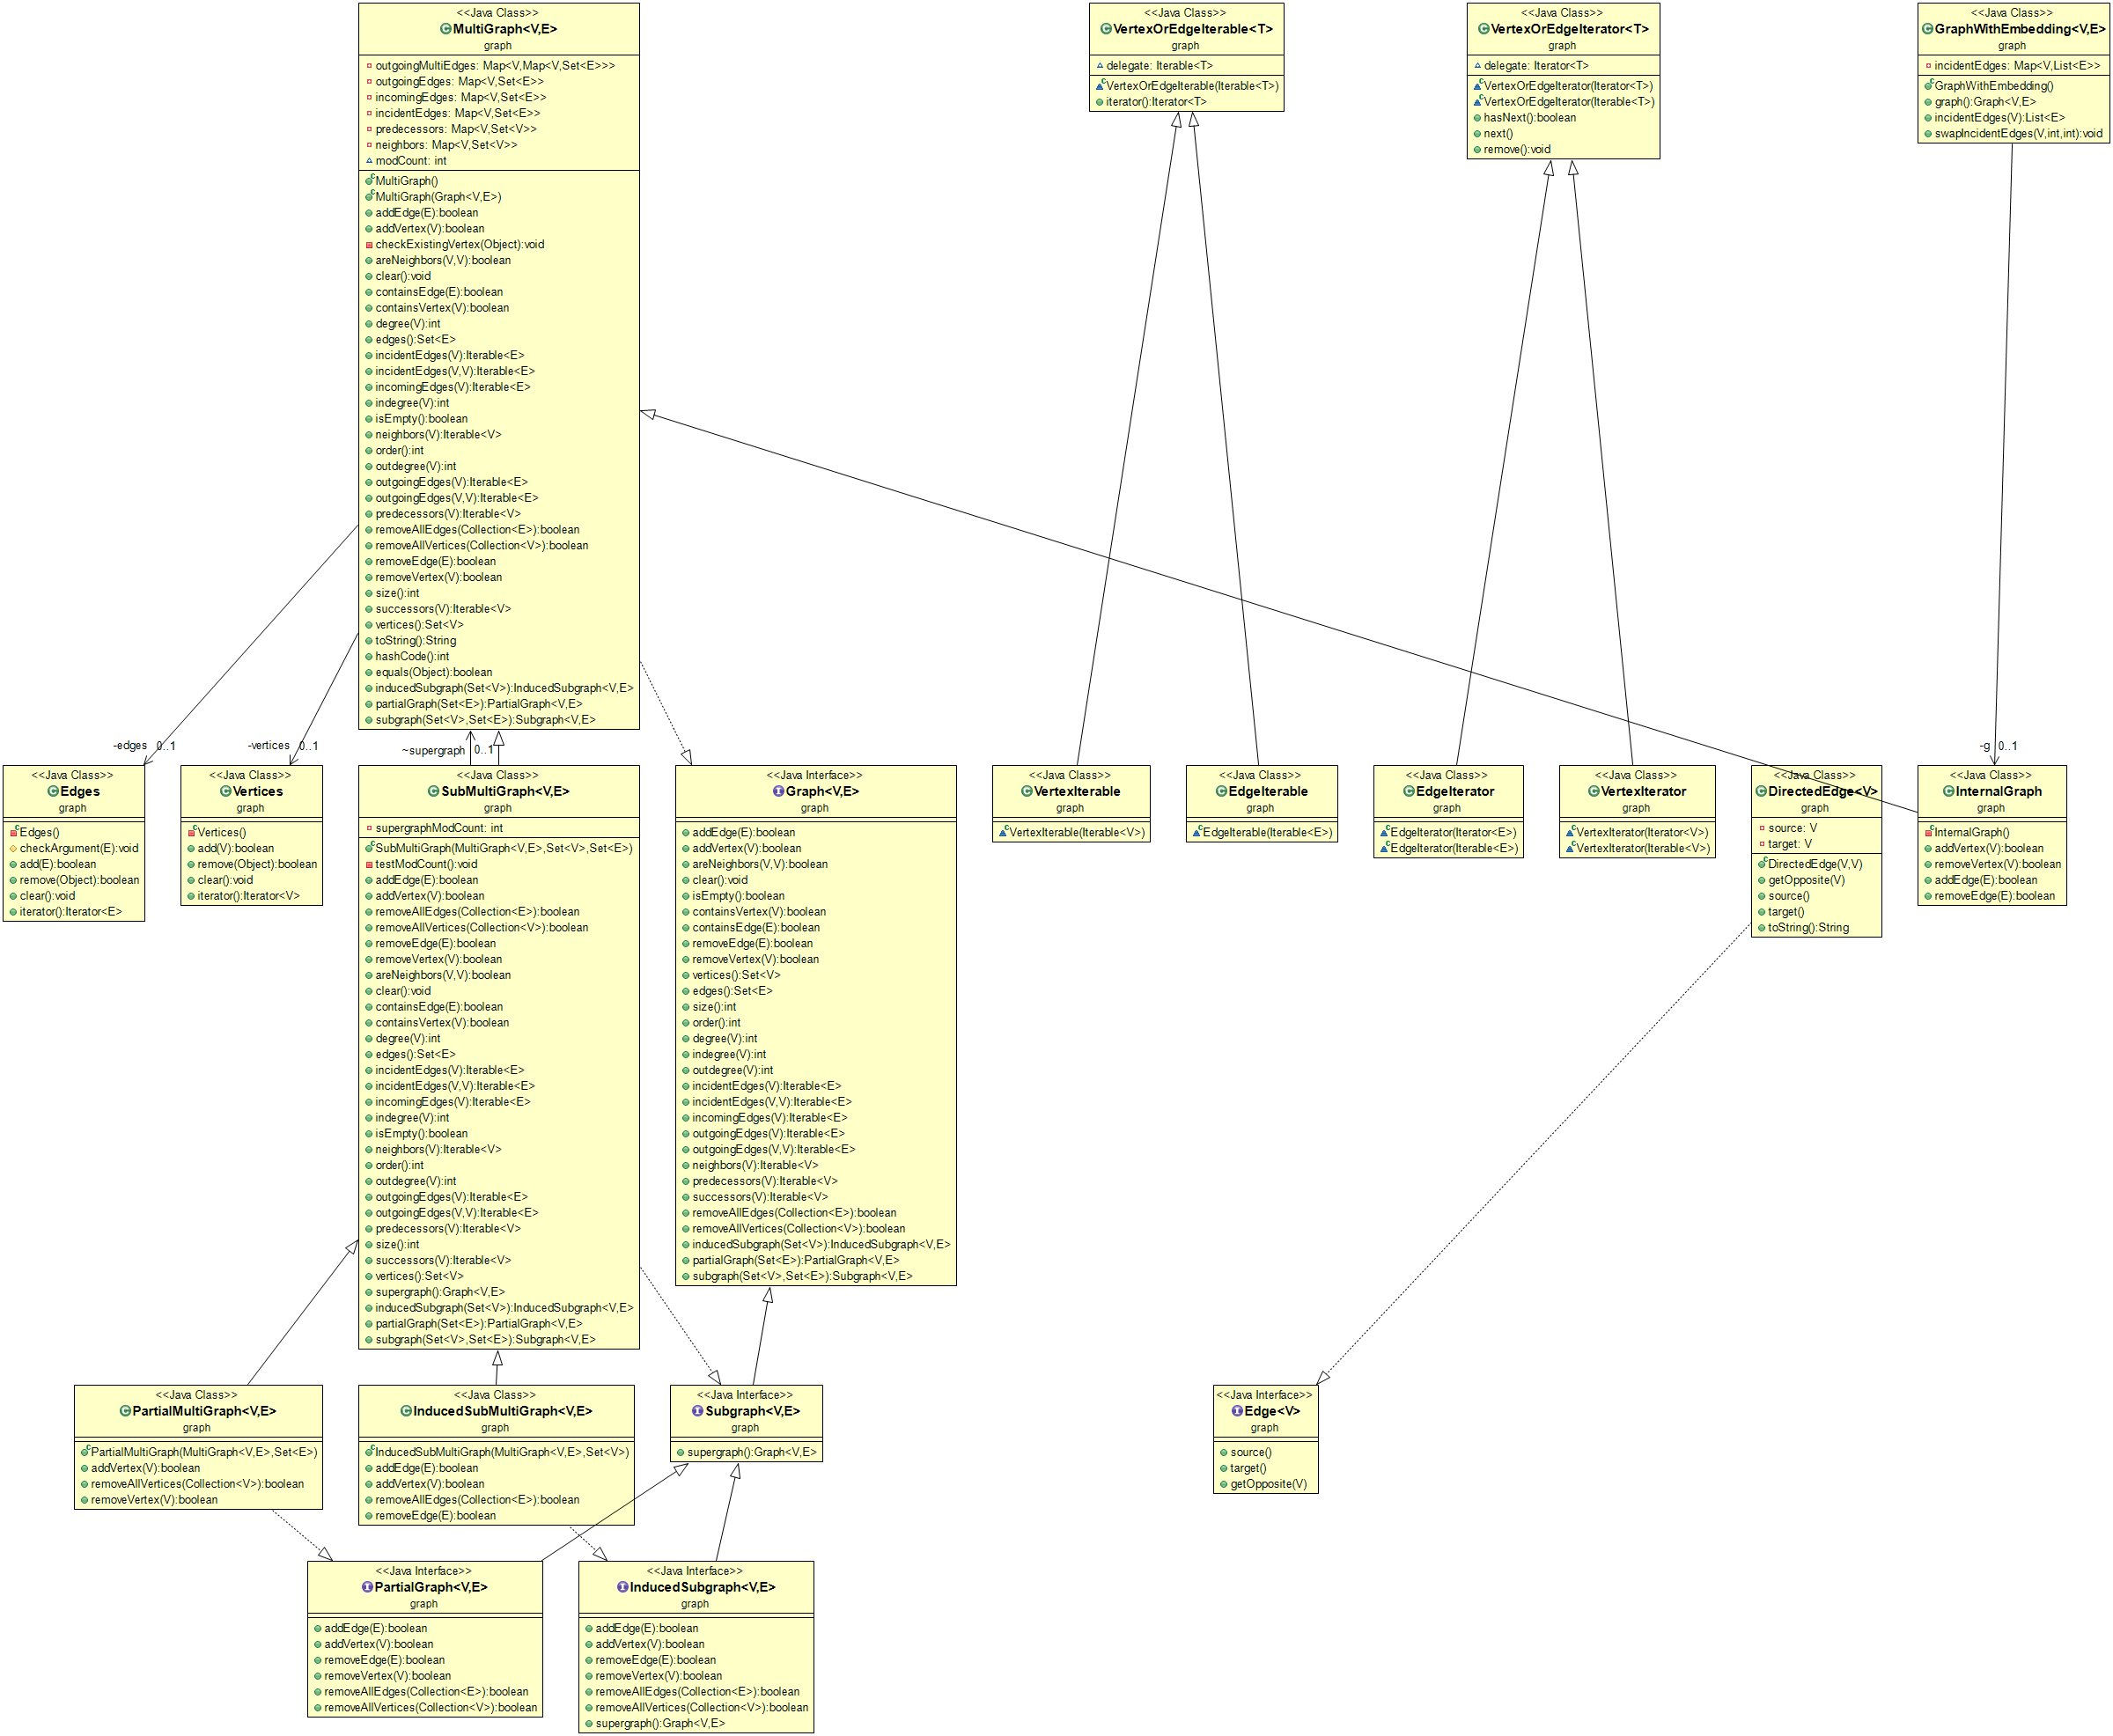
\includegraphics[height = 3in]{3packagegraph.png}
		\caption[Optional caption]{Package Graph}
		\label{fig:1main}
	\end{figure}
	%Figure \ref{fig:3packagegraph} The Graph
	
	\begin{figure}[H]
		\centering
		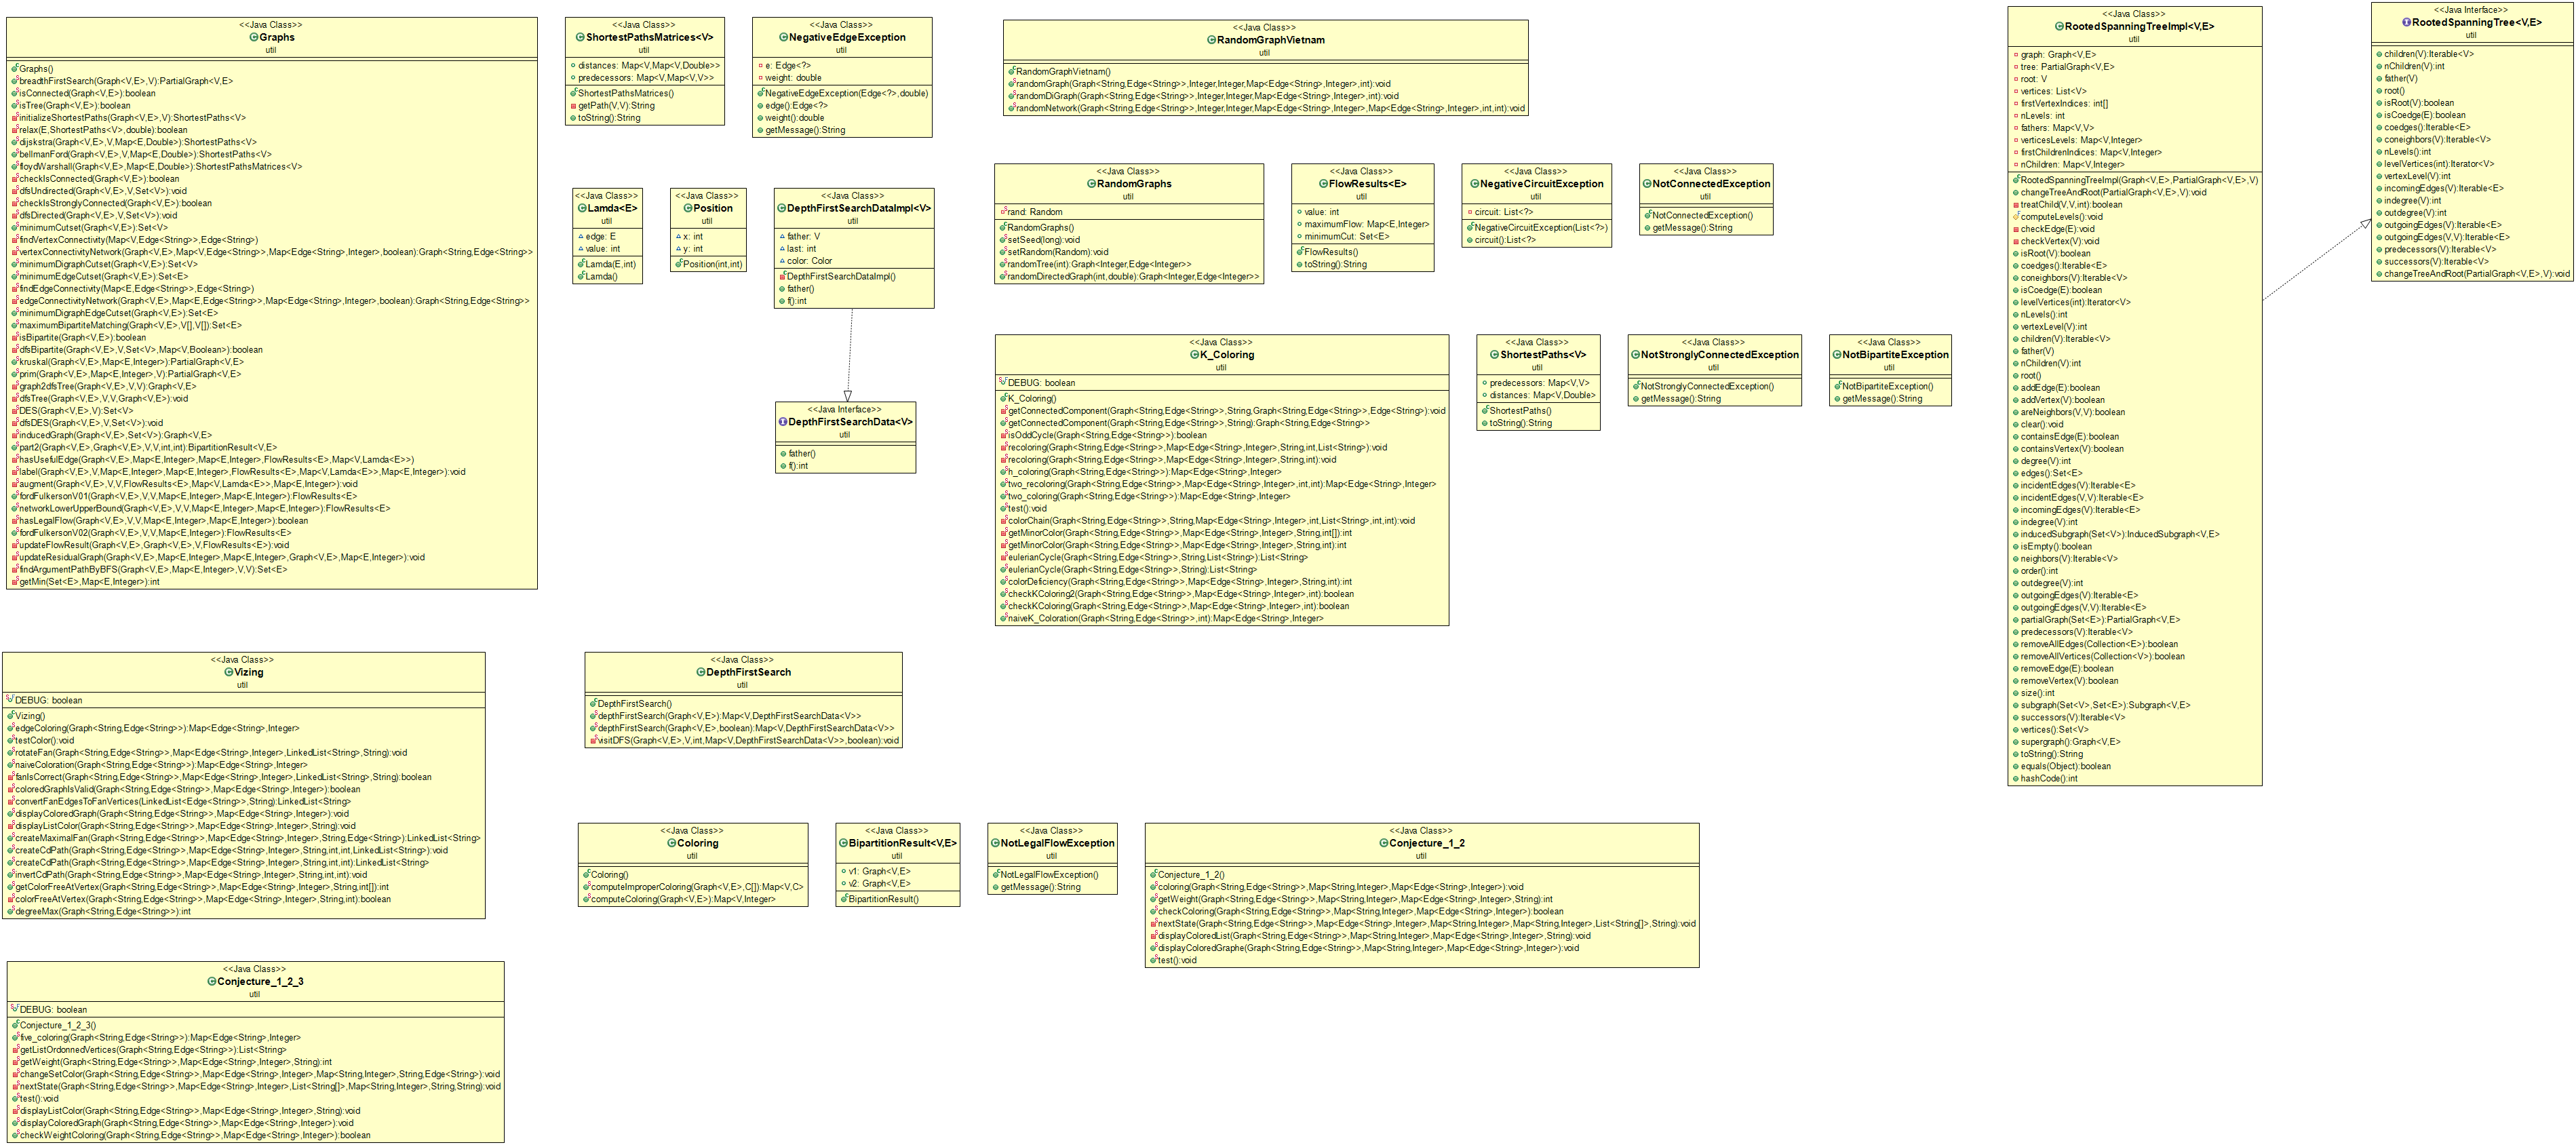
\includegraphics[height = 3in]{4packageutil.png}
		\caption[Optional caption]{Package Util}
		\label{fig:1main}
	\end{figure}
	%Figure \ref{fig:4packageutilh} The Graph
\subsubsection{User Interface}
\begin{figure}[H]
		\centering
		
\includegraphics[height = 3in]{graph.png}
		\caption[Optional caption]{User Interface}
		\label{fig:1main}
	\end{figure}
	%Figure \ref{fig:4packageutilh} The Graph
%
%Architecture
\section{Architecture}
\subsection{Introduction}
This document provides a high level overview and explains the architecture of Graph Application.
The document defines goals of the architecture, the use cases supported by the system, architectural styles and components that have been selected. The document provides a rationale for the architecture and design decisions made from the conceptual idea to its implementation. 
\subsubsection{Purpose}
The Software Architecture Document (SAD) provides a comprehensive architectural overview of the Graph Application It presents a number of different architectural views to depict the different aspects of the system.  
\subsubsection{Scope}
The scope of this SAD is to explain the architecture of the Graph Application.
This document describes the various aspects of the Graph application design that are considered to be architecturally significant. These elements and behaviors are fundamental for guiding the construction of the Graph application and for understanding this project as a whole.

\subsection{Architectural Representation}
\subsubsection{Use Case view}
Audience: all the stakeholders of the system, including the end-users.
\paragraph{}
Area: describes the set of scenarios and/or use cases that represent some significant, central functionality of the system. Describes the actors and use cases for the system, this view presents the needs of the user and is elaborated further at the design level to describe discrete flows and constraints in more detail. This domain vocabulary is independent of any processing model or representational syntax (i.e. XML).
\subsubsection{Logical view}
Audience: Designers.
\paragraph{}
Area: Functional Requirements: describes the design's object model. Also describes the most important use-case realizations and business requirements of the system.
\paragraph{}
Related Artifacts: Design model

\subsection{Architectural Goals and Constraints}
There are some key requirements and system constraints that have a significant bearing on the architecture.  They are:
\paragraph{}
1.	The system is meant as a proof of concept for a more complete project prediction system to be built in the future.  Therefore one of the primary stakeholders in this document and the system as a whole are future architects and designers, not necessarily users as is normally the case.  As a result, one goal of this document is to be useful to future architects and designers.
\paragraph{}
2.	The system will be written using JAVA 8 technologies but will use an open source JavaFX for Design Graphic user interface and will be runable to operating system with Java Virtual Machine be installed.
\paragraph{}
3.	The Application may be reference to the third-party for graph such as JGraphT.


\subsection{Use-Case Realizations}
\subsubsection{Find the shortest path of graph}
\begin{figure}[H]
		\centering
		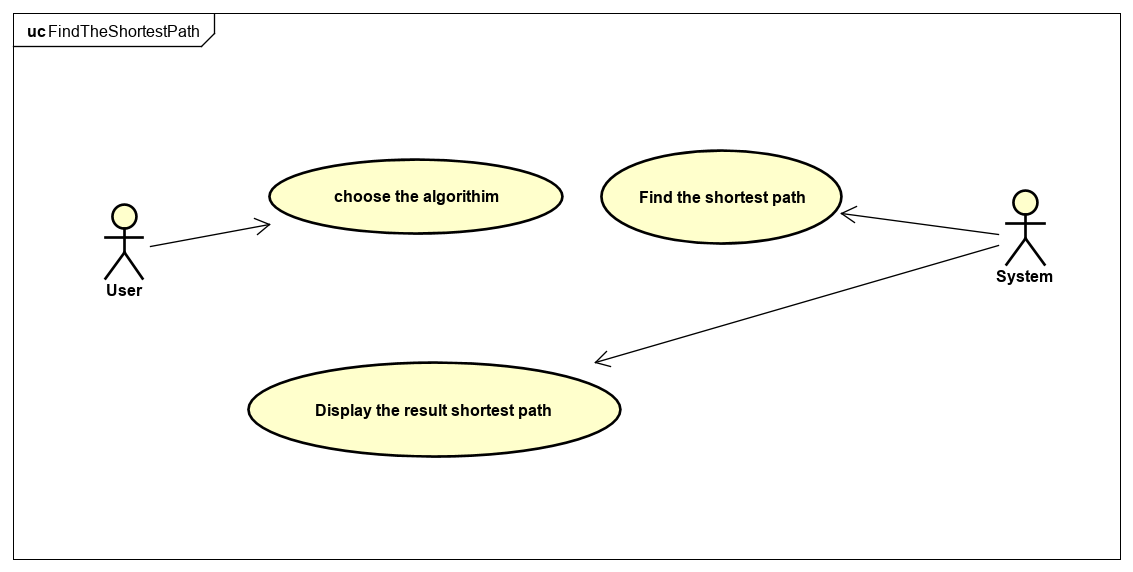
\includegraphics[height = 3in]{usecase_findshortestpath.png}
		\caption[Optional caption]{Find the shortest path of graph}
		\label{fig:usecase_findshortestpath}
	\end{figure}
	%Figure \ref{fig:image1} The Graph
	
	\begin{figure}[H]
		\centering
		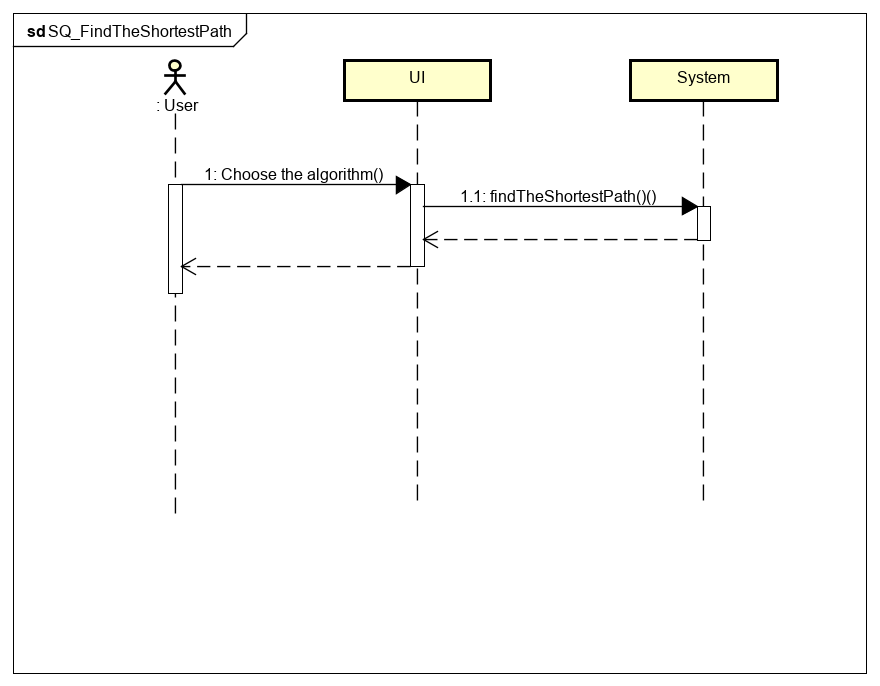
\includegraphics[height = 3in]{SQ_FindTheShortestPath.png}
		\caption[Optional caption]{Sequence FindTheShortestPath}
		\label{fig:usecase_findshortestpath}
	\end{figure}
	%Figure \ref{fig:image1} The Graph
\subsubsection{Draw Vertices}
\begin{figure}[H]
		\centering
		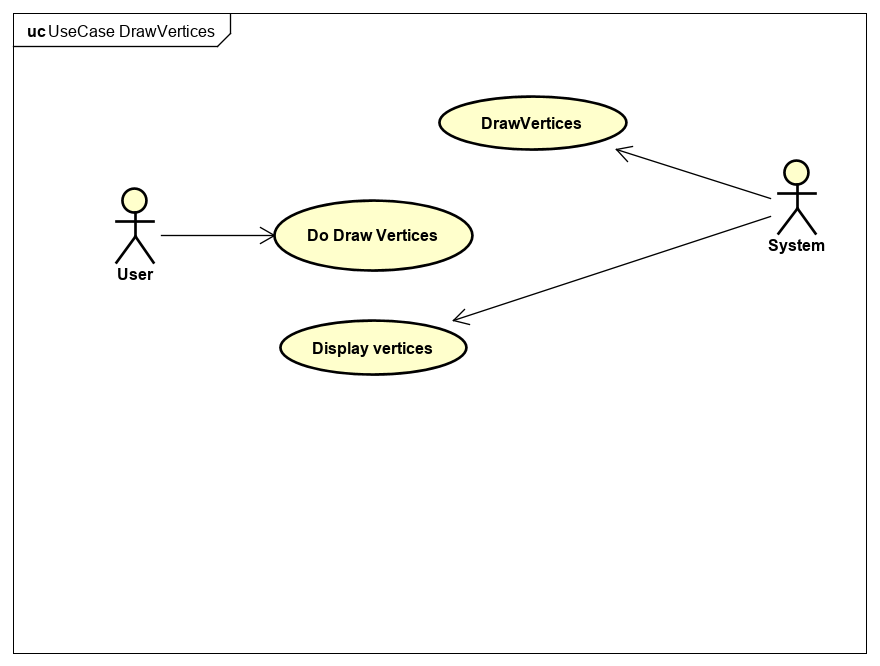
\includegraphics[height = 3in]{UseCaseDrawVertices.png}
		\caption[Optional caption]{UseCaseDrawVertices}
		\label{fig:UseCaseDrawVertices}
	\end{figure}
	%Figure \ref{fig:image1} The Graph
	
	\begin{figure}[H]
		\centering
		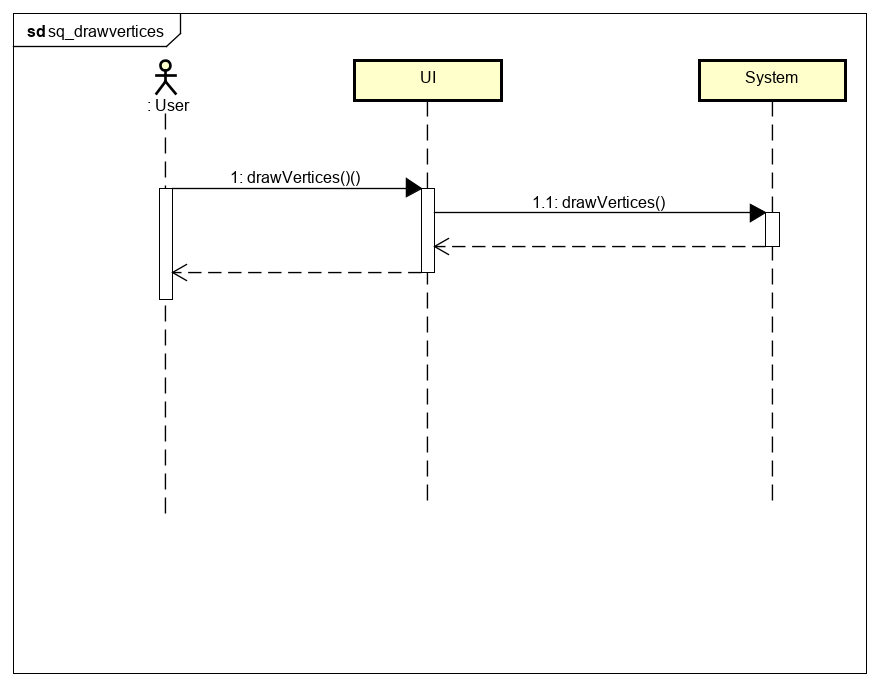
\includegraphics[height = 3in]{sq_drawvertices.png}
		\caption[Optional caption]{Sequence drawvertices}
		\label{fig:Sequence_drawvertices}
	\end{figure}
	%Figure \ref{fig:image1} The Graph
	
\subsubsection{Draw Edges}
\begin{figure}[H]
		\centering
		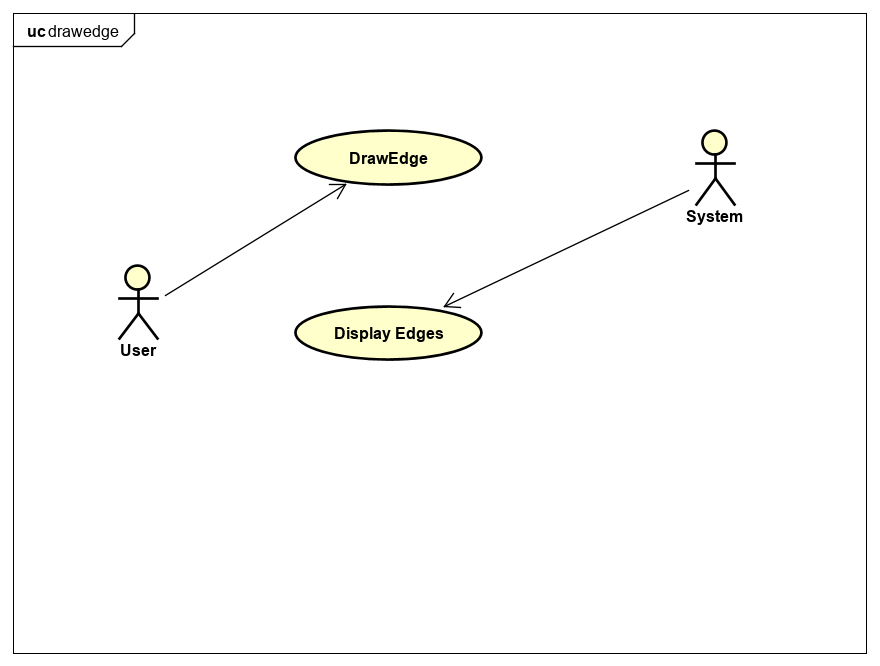
\includegraphics[height = 3in]{UseCaseDrawEdge.png}
		\caption[Optional caption]{UseCaseDrawEdge}
		\label{fig:UseCaseDrawEdge}
	\end{figure}
	%Figure \ref{fig:image1} The Graph
	
	\begin{figure}[H]
		\centering
		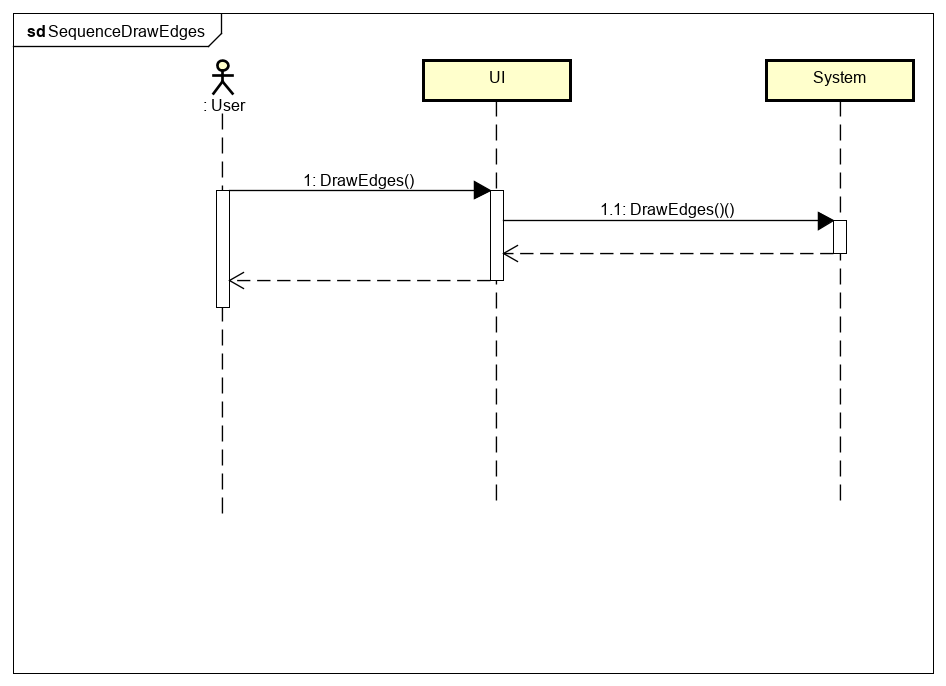
\includegraphics[height = 3in]{SequenceDrawEdges.png}
		\caption[Optional caption]{SequenceDrawEdges}
		\label{fig:SequenceDrawEdges}
	\end{figure}
	%Figure \ref{fig:image1} The Graph
	
\subsubsection{Delete Edges}
\begin{figure}[H]
		\centering
		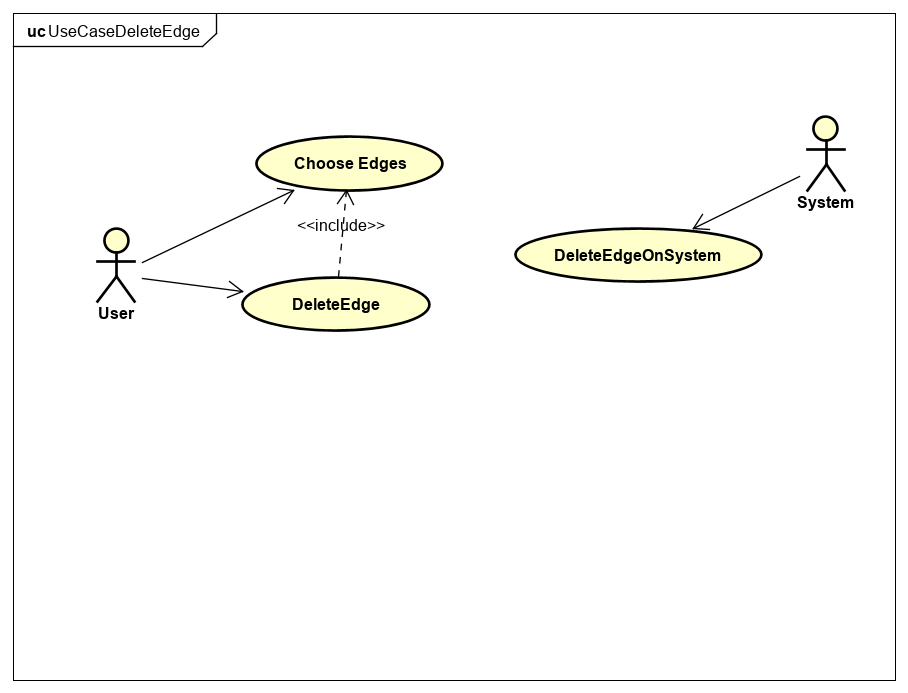
\includegraphics[height = 3in]{UseCaseDeleteEdge.png}
		\caption[Optional caption]{UseCaseDeleteEdge}
		\label{fig:UseCaseDeleteEdge}
	\end{figure}
	%Figure \ref{fig:image1} The Graph
	
	\begin{figure}[H]
		\centering
		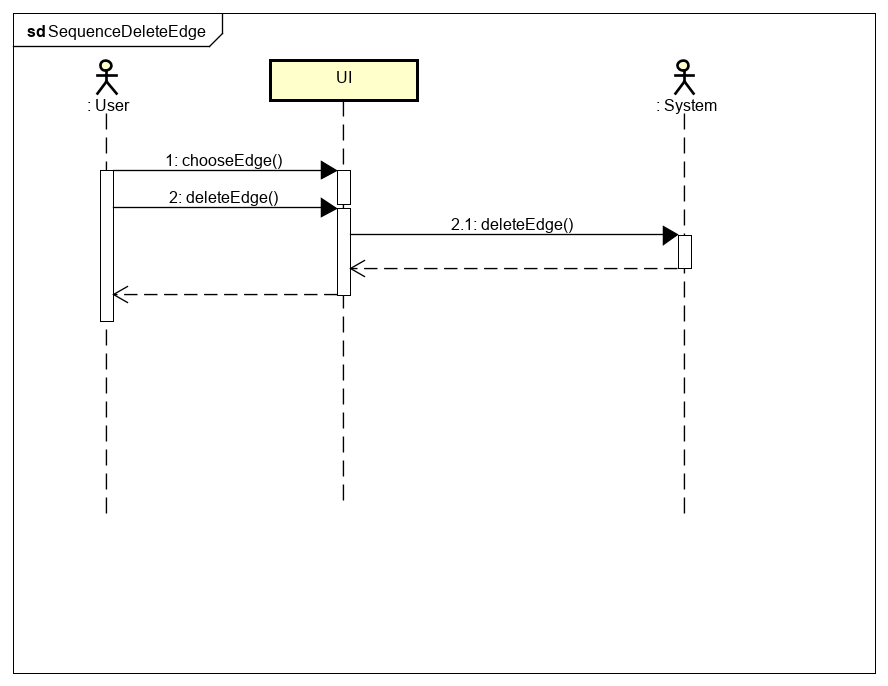
\includegraphics[height = 3in]{SequenceDeleteEdge.png}
		\caption[Optional caption]{SequenceDeleteEdge}
		\label{fig:SequenceDeleteEdge}
	\end{figure}
	%Figure \ref{fig:image1} The Graph
	
\subsubsection{Delete Vertices}
\begin{figure}[H]
		\centering
		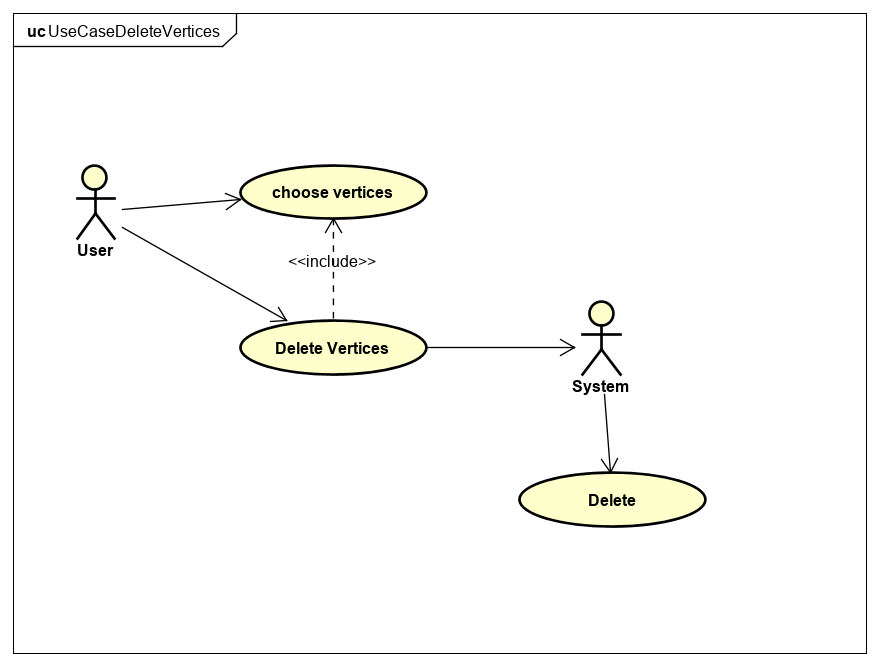
\includegraphics[height = 3in]{UseCaseDeleteVertices.png}
		\caption[Optional caption]{UseCaseDeleteVertices}
		\label{fig:UseCaseDeleteVertices}
	\end{figure}
	%Figure \ref{fig:image1} The Graph
	
	\begin{figure}[H]
		\centering
		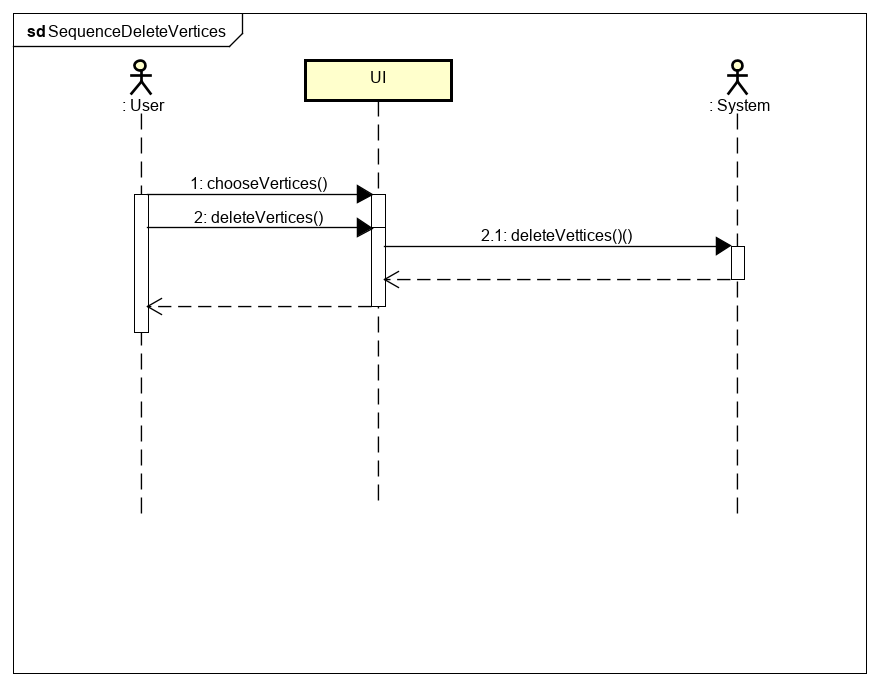
\includegraphics[height = 3in]{SequenceDeleteVertices.png}
		\caption[Optional caption]{SequenceDeleteVertices}
		\label{fig:SequenceDeleteVertices}
	\end{figure}
	%Figure \ref{fig:image1} The Graph
	
\subsubsection{Move Vertices}
\begin{figure}[H]
		\centering
		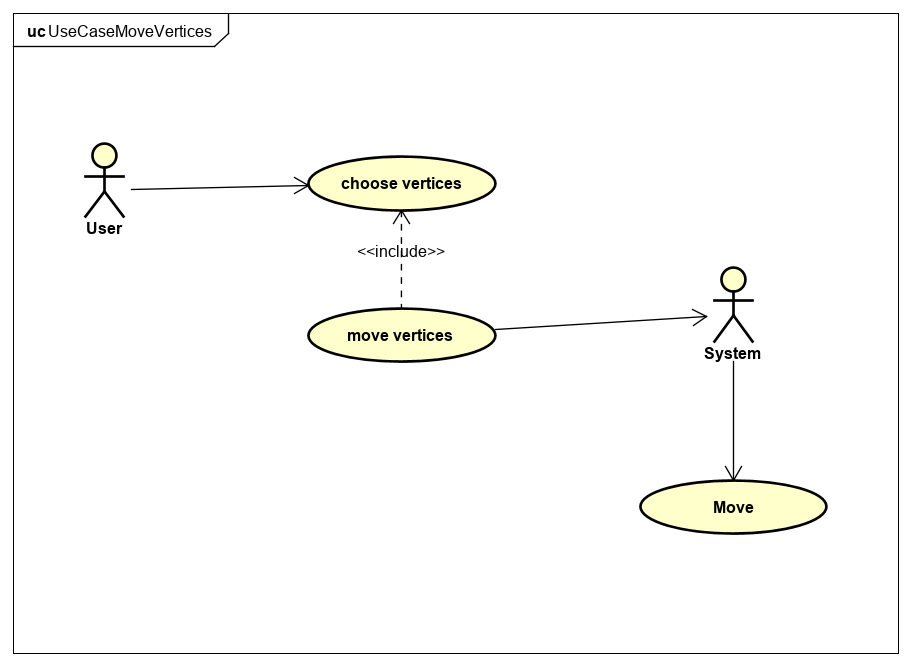
\includegraphics[height = 3in]{UseCaseMoveVertices.png}
		\caption[Optional caption]{UseCaseMoveVertices}
		\label{fig:UseCaseMoveVertices}
	\end{figure}
	%Figure \ref{fig:image1} The Graph
	
	\begin{figure}[H]
		\centering
		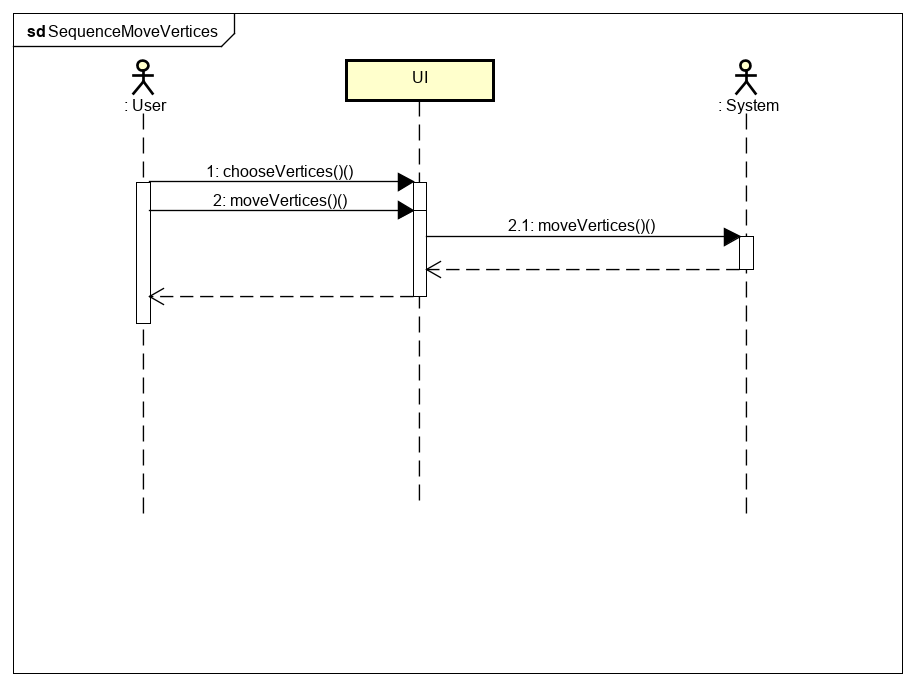
\includegraphics[height = 3in]{SequenceMoveVertices.png}
		\caption[Optional caption]{SequenceMoveVertices}
		\label{fig:SequenceMoveVertices}
	\end{figure}
	%Figure \ref{fig:image1} The Graph
%


%application
\section{Application}
\subsection{Git Hub}
\subsubsection{Repository}
 Repository: https://github.com/nhat2211/GraF.git
 \begin{figure}[H]
		\centering
		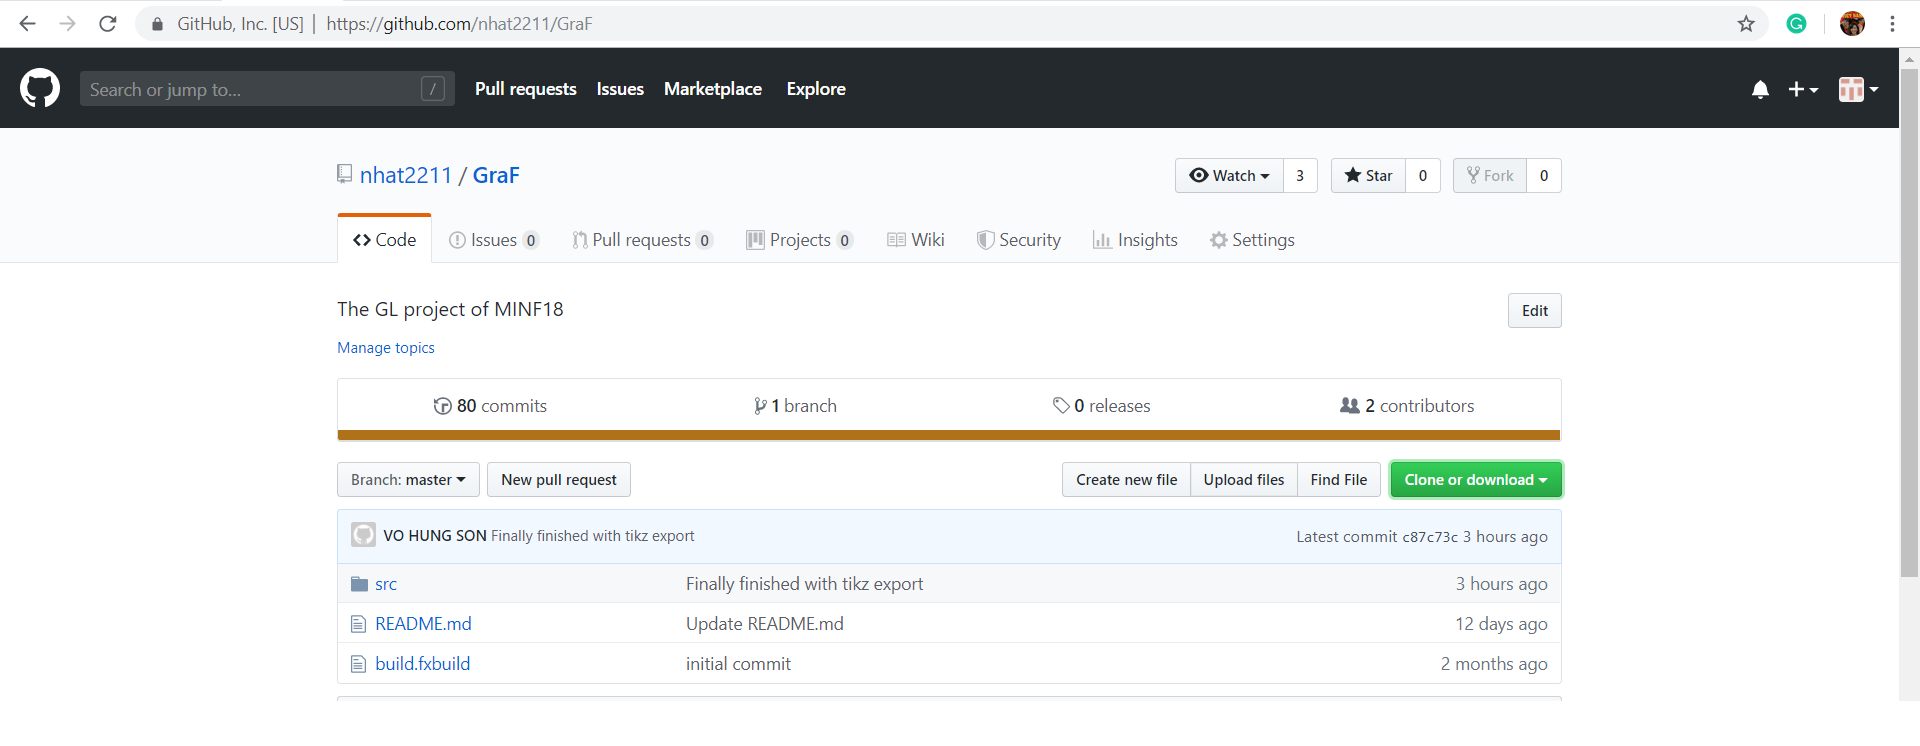
\includegraphics[height = 3in]{gitImage.png}
		\caption[Optional caption]{Repository}
		\label{fig:Repository}
	\end{figure}
	%Figure \ref{fig:gitImage} The Graph
\paragraph{}
\subsection{Requirement} 
The GL project of MINF18 here is a set of requests for the project :

1- create a gitHub project with name GraF (for Graph Framework). My login in gitHub is baudon (for the invitation) and the associated adress olivier.baudon@labri.fr Please tell me each time you want that I take a look on your code.

2- Provide an interface which allow to create graphs where a vertex is represented by a circle and an edge by a straight line.

3- Give the possibility to move vertices.

4- Give the possibility to change the form of the vertices and the edges (arc, or segments with intermediate points movable by the user), and to have oriented edges.

5- Give the possibility to suppress a vertex or an edge.

6- Add labels to vertices and edges.

7- Give the possibility to the user to change the position of the labels, and the value of the labels.

Remark : I propose that you provide a toolbar on the left side of the window to propose the different types of vertices and edges and to change the effect of a click (for example, an icon with scissors (or death's head) means supress, an icon with a cross means add an intermediate point to an edge, ...)

For each version, you may also provide the tkz version of the drawing, using a menu for the export.
\subsection{Architecture} 
We use Model-View-Controller in the application development.
\begin{figure}[H]
		\centering
		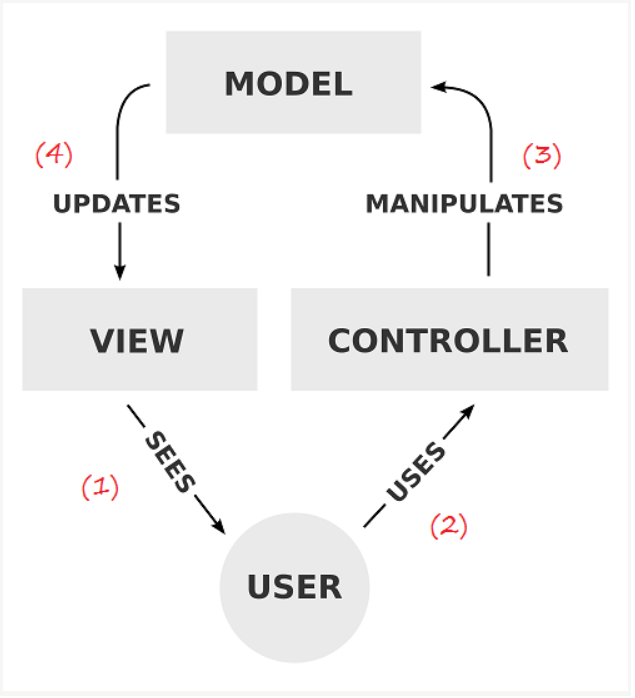
\includegraphics[height = 3in]{mvc.png}
		\caption[Optional caption]{Model-View-Controller}
		\label{fig:Repository}
	\end{figure}
	%Figure \ref{fig:gitImage} The Graph
\paragraph{}
1. After that the user see on \textbf{VIEW}
\paragraph{}
2. User use \textbf{CONTRONLLER}
\paragraph{}
3. Apply data (Update,edit,delete,etc..), data on \textbf{MODEL} changed
\paragraph{}
4. Display data of \textbf{MODEL} on \textbf{VIEW}

\paragraph{}
\begin{figure}[H]
		\centering
		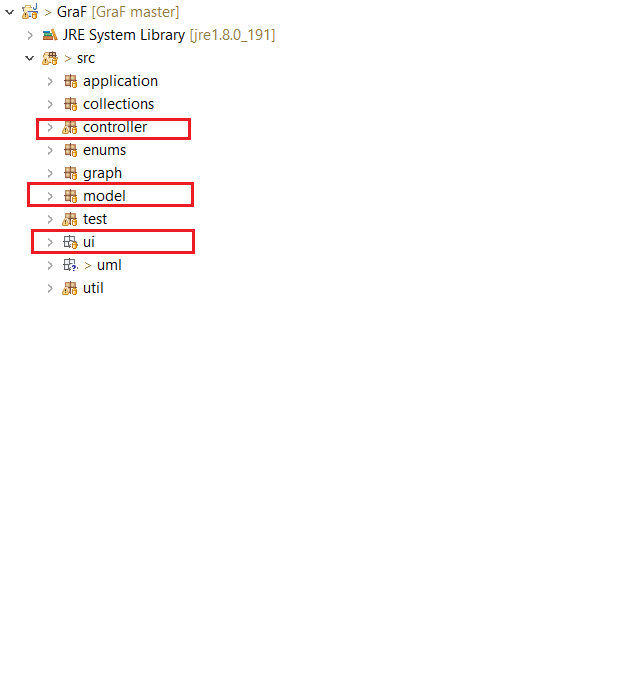
\includegraphics[height = 3in]{structure.png}
		\caption[Optional caption]{Model-View-Controller Project Structure}
		\label{fig:Repository}
	\end{figure}
	%Figure \ref{fig:gitImage} The Graph
\paragraph{}


\subsection{Framework} 
Why choose JavaFX for Developing Application?:

Our experience proves that implementing an employee desktop front end with native technology is a valid approach and that JavaFX is a good fit.
\begin{itemize}
	\item JavaFX is available on the leading desktop operating systems (Windows, Linux, and . Mac OS X).
	\item Although it has gone through some painful changes, its evolution proves its       vendor's level of commitment.
	\item As the successor to Swing, it is being used by an increasing number of Java developers. Regardless of its future, it will benefit from a strong developer community.
	\item Compared to Swing, it provides a clear and clean architecture and features many enhancements: styling, event management, transitions, scene graph—to name a few.
	\item It provides the possibility of developing up-to-date user interfaces with animations, multitouch, and the like.
	\item It is based on a clear and clean language: Java.
	\item It provides all the professional Java tooling required to debug, analyze, profile, and log a client application.
	\item It enables a simple app-like installation on the client side, without any prerequisites.
	\item In short, we believe that JavaFX is the only native UI environment that provides all these features today.
\end{itemize}

Source: https://www.oracle.com/technetwork/articles/java/casa-1919152.html
\paragraph{}




\subsection{UML} 

1. Class Diagram:
\paragraph{}
\begin{figure}[H]
		\centering
		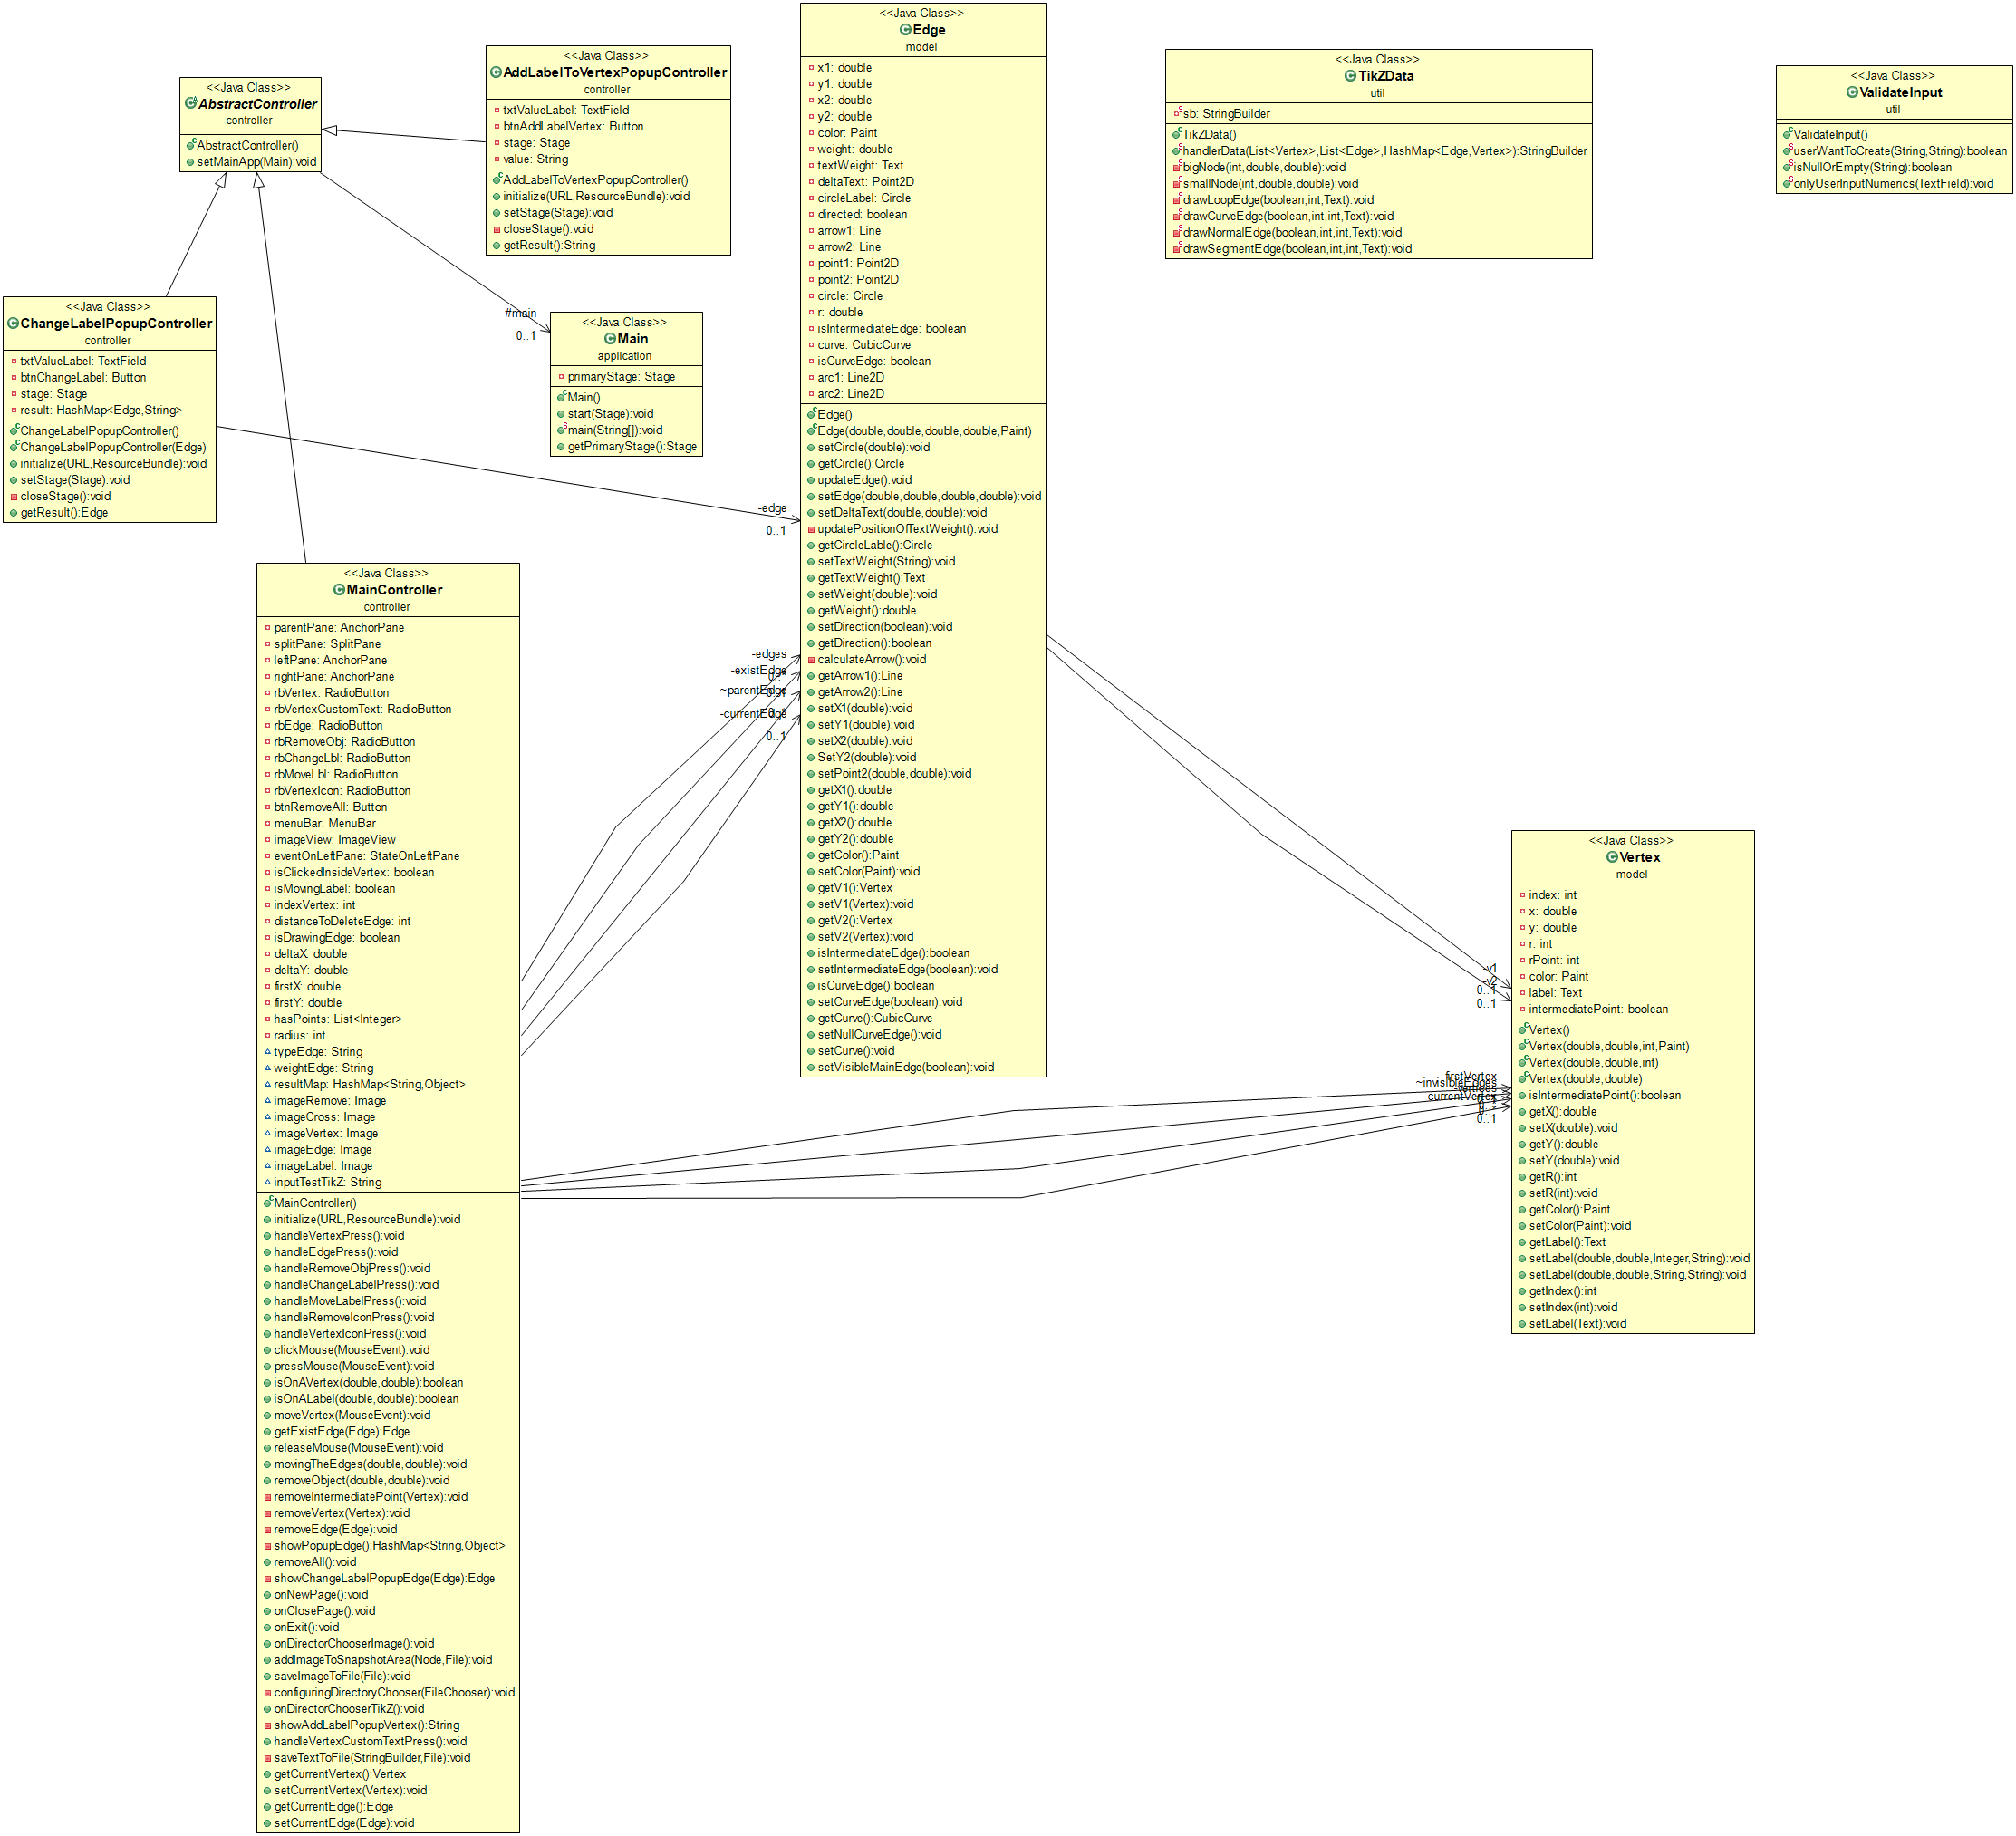
\includegraphics[height = 3in]{class_diagram.png}
		\caption[Optional caption]{Class Diagram}
		\label{fig:Repository}
	\end{figure}
	%Figure \ref{fig:gitImage} The Graph
\paragraph{}

\subsection{IDE} 

Eclipse

\subsection{Unit Test} 
\begin{enumerate}
	\item One
	\item Two
	\item Three
\end{enumerate}
Junit 4
\subsection{Functions} 
\subsubsection{Draw vertex}
	\begin{tabular}{|r|l|}
\hline
Name: & Draw Vertices \\
\hline
Actor & User \\
\hline
Entry Conditions: & Application is running. \\
\hline
Flow of Events: & 1. User choose vertex option on left pane. \\


& 2. System remember the type which user chose.  \\
& 3. User press mouse left button on panel.  \\
& 4. System will draw a vertice on the panel by a circle.  \\
\hline
Exit Conditions: & The application is now in a new state. \\
\hline

\end{tabular}
	\paragraph{}
	
\begin{figure}[H]
		\centering
		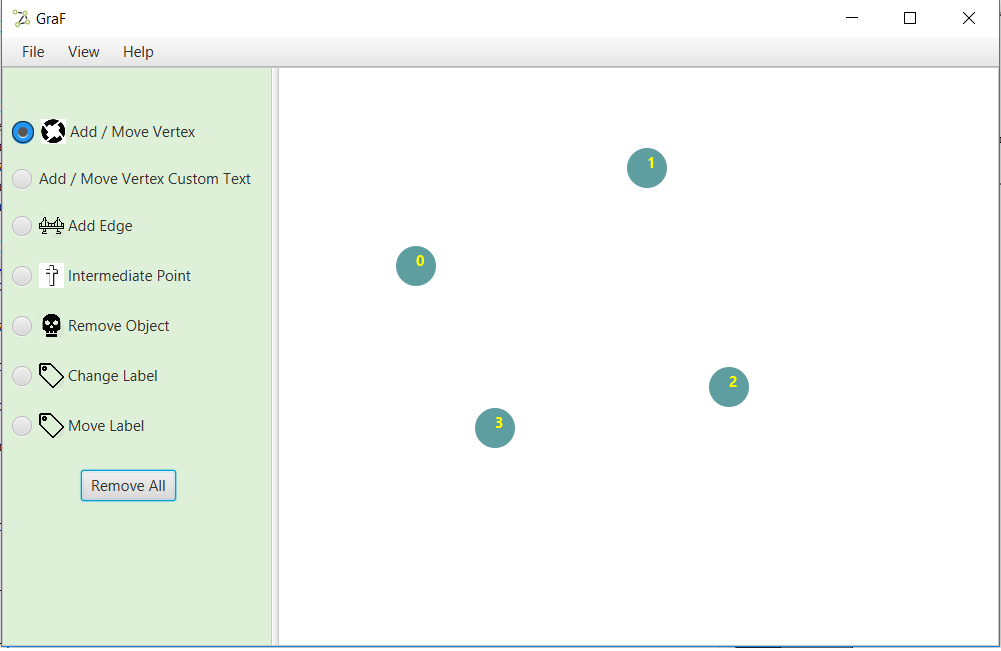
\includegraphics[height = 3in]{drawVertex.png}
		\caption[Optional caption]{Draw vertex}
		\label{fig:Repository}
	\end{figure}
	%Figure \ref{fig:gitImage} The Graph
\paragraph{}
\subsubsection{Draw vertex custom text}
	\begin{tabular}{|r|l|}
\hline
Name: & Draw vertex custom text \\
\hline
Actor & User \\
\hline
Entry Conditions: & Application is running. \\
\hline
Flow of Events: & 1. User choose vertex custom text option on left pane. \\


& 2. System remember the type which user chose.  \\
& 3. User press mouse left button on panel.  \\
& 4. The popup add vertex be showed  \\
& 5. User type text in textbox  \\
& 6. User click add button  \\
& 7. System draw a vertex with label be text which user input   \\
\hline
Exit Conditions: & The application is now in a new state. \\
\hline

\end{tabular}
	\paragraph{}
	
\begin{figure}[H]
		\centering
		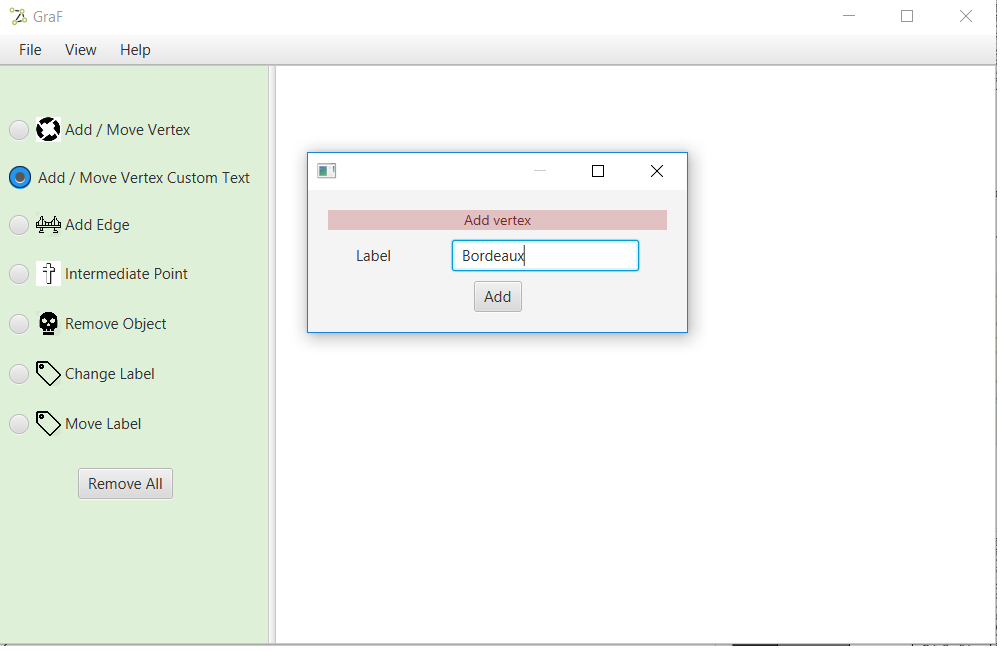
\includegraphics[height = 3in]{drawVertexWithText.png}
		\caption[Optional caption]{Draw vertex with text}
		\label{fig:Repository}
	\end{figure}
	%Figure \ref{fig:gitImage} The Graph
\paragraph{}
\begin{figure}[H]
		\centering
		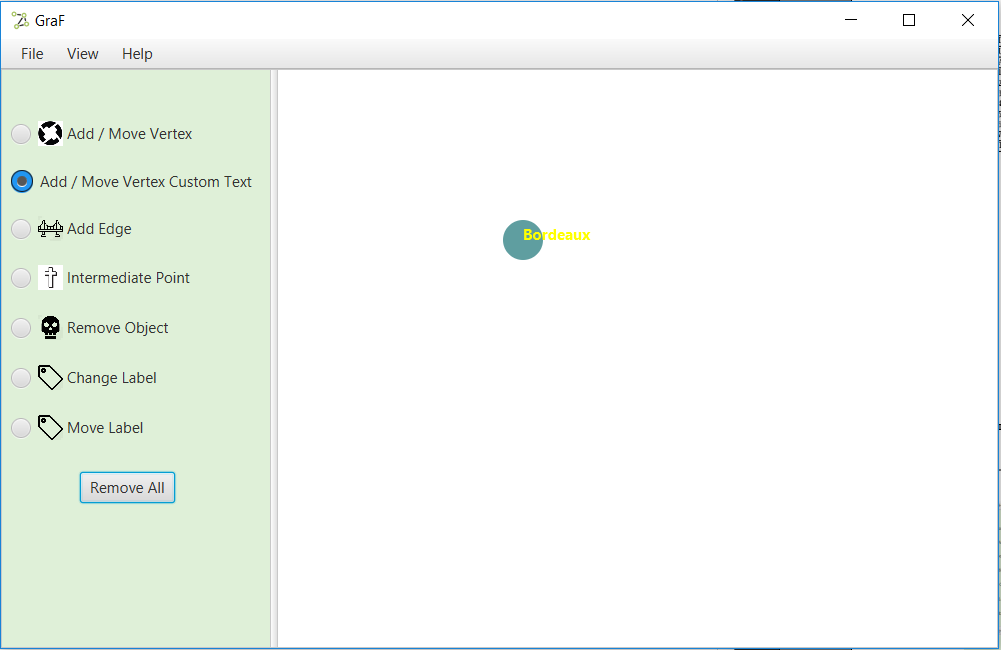
\includegraphics[height = 3in]{drawVertexWithText2.png}
		\caption[Optional caption]{Draw vertex with text}
		\label{fig:Repository}
	\end{figure}
	%Figure \ref{fig:gitImage} The Graph
%

\subsubsection{Move vertex}
	\begin{tabular}{|r|l|}
\hline
Name: & Move Vertex \\
\hline
Actor & User \\
\hline
Entry Conditions: & Existing at least one vertex for moving. \\
\hline
Flow of Events: & 1. User choose move vertex option on left pane. \\
& 2. System remember the type which user chose.  \\
& 3. User press and hold mouse left button on vertex.  \\
& 4. User hold press the left mouse on the vertex and move the mouse for moving vertex.  \\
\hline
Exit Conditions: & The application is now in a new state. \\
\hline

\end{tabular}
	\paragraph{}
	
\begin{figure}[H]
		\centering
		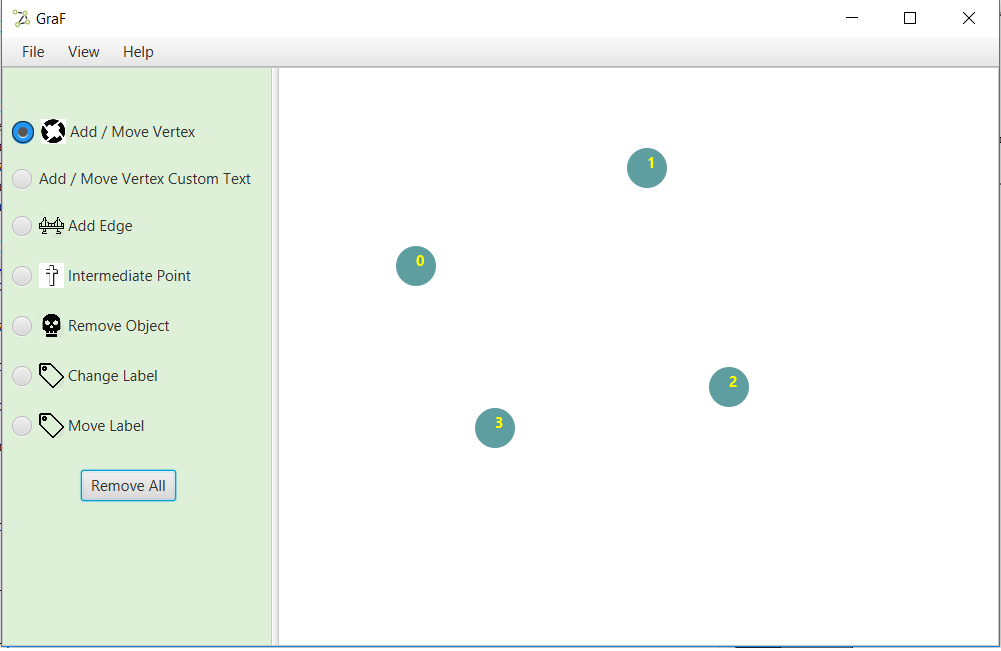
\includegraphics[height = 3in]{drawVertex.png}
		\caption[Optional caption]{Move vertex}
		\label{fig:Repository}
	\end{figure}
	%Figure \ref{fig:gitImage} The Graph
\paragraph{}

\subsubsection{Draw edge}
	\begin{tabular}{|r|l|}
\hline
Name: & Draw edge \\
\hline
Actor & User \\
\hline
Entry Conditions: & Existing two at least two vertex on right pane. \\
\hline
Flow of Events: & 1. User choose add edge option on left pane. \\
& 2. System remember the type which user chose.  \\
& 3. User press and hold left mouse on the first vertex.  \\
& 4. User hold press left mouse and move cursor to inside the second vertex.  \\
& 5. User release mouse.  \\
& 6. The popup Add edge be showed.  \\
& 7. User input the weight of edge.  \\
& 8. User click Directed button or Undirected button for create edge   \\
& 9. System draw a edge.   \\
\hline
Exit Conditions: & The application is now in a new state. \\
\hline

\end{tabular}
	\paragraph{}
	
\begin{figure}[H]
		\centering
		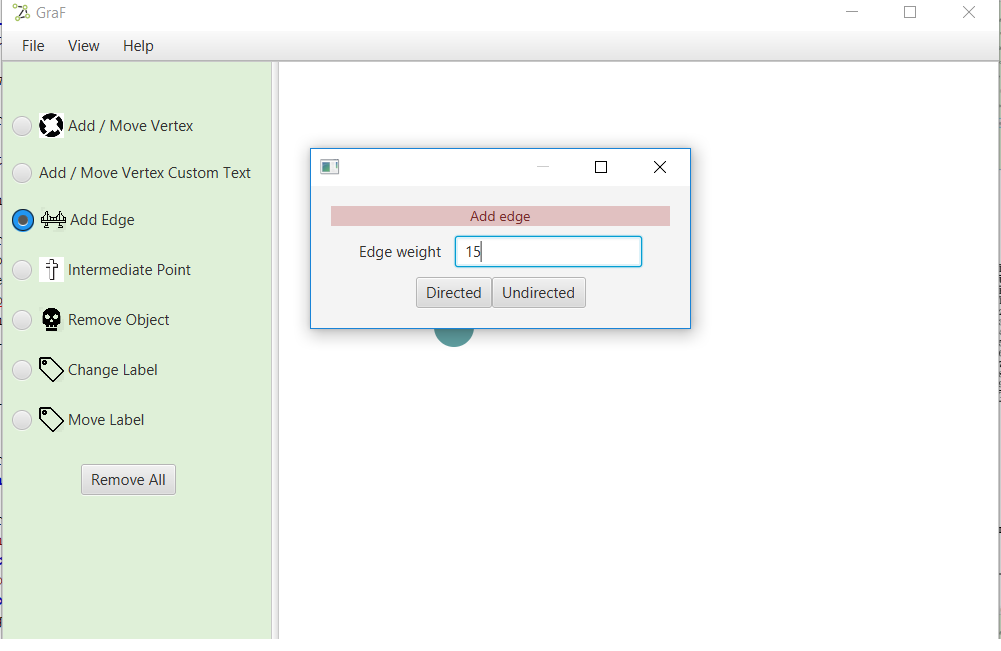
\includegraphics[height = 3in]{addEdge1.png}
		\caption[Optional caption]{Add edge}
		\label{fig:Repository}
	\end{figure}
	%Figure \ref{fig:gitImage} The Graph
\paragraph{}

\begin{figure}[H]
		\centering
		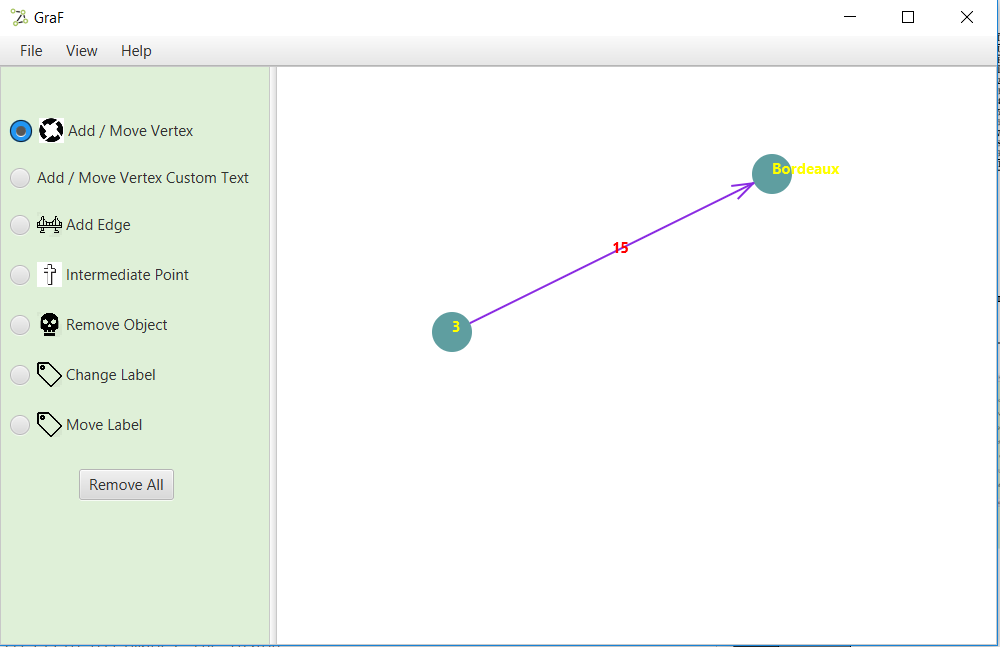
\includegraphics[height = 3in]{addEdge2.png}
		\caption[Optional caption]{Add edge}
		\label{fig:Repository}
	\end{figure}
	%Figure \ref{fig:gitImage} The Graph
\paragraph{}

\subsubsection{Intermediate Point}
	\begin{tabular}{|r|l|}
\hline
Name: & Intermediate Point \\
\hline
Actor & User \\
\hline
Entry Conditions: & Existing at least one edge on right pane. \\
\hline
Flow of Events: & 1. User choose Intermediate Point option on left pane. \\
& 2. System remember the type which user chose.  \\
& 3. User press left mouse on a edge  \\
& 4. System draw a Intermediate Point on this edge  \\
\\
\hline
Exit Conditions: & The application is now in a new state. \\
\hline

\end{tabular}
	\paragraph{}
	
\begin{figure}[H]
		\centering
		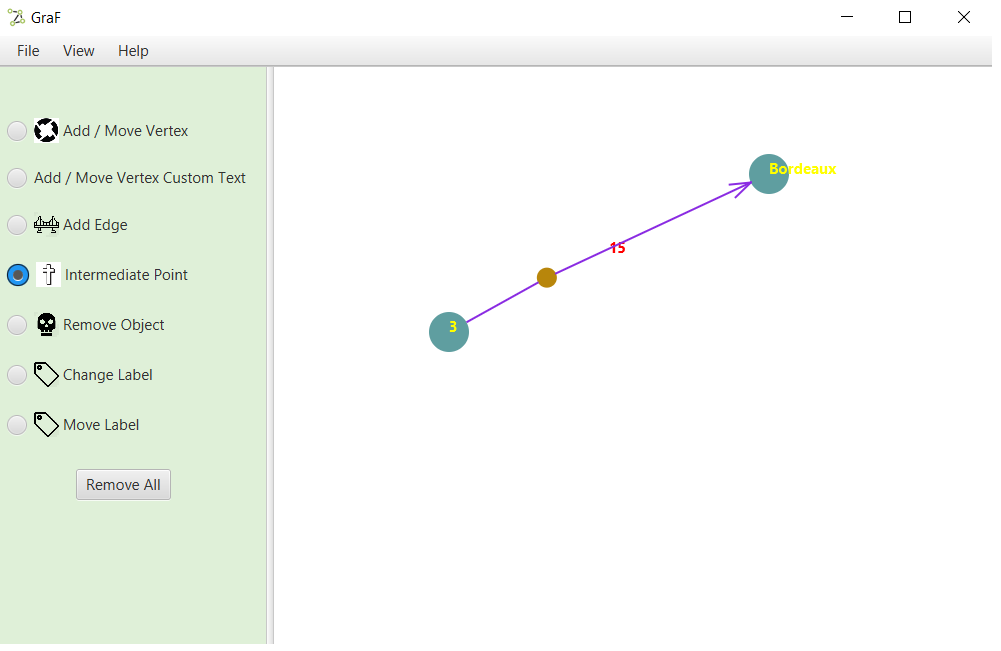
\includegraphics[height = 3in]{IntermediatePoint.png}
		\caption[Optional caption]{Intermediate Point}
		\label{fig:Repository}
	\end{figure}
	%Figure \ref{fig:gitImage} The Graph
\paragraph{}

\subsubsection{Remove Object}
	\begin{tabular}{|r|l|}
\hline
Name: & Remove Object \\
\hline
Actor & User \\
\hline
Entry Conditions: & Existing at least one object on right pane. \\
\hline
Flow of Events: & 1. User choose Remove Object option on left pane. \\
& 2. System remember the type which user chose.  \\
& 3. User press left mouse on a object  \\
& 4. System remove object  \\
\\
\hline
Exit Conditions: & The application is now in a new state. \\
\hline

\end{tabular}
	\paragraph{}

\newpage
\addcontentsline{toc}{section}{\numberline{}References}
\printbibliography
\end{document}
